\documentclass{acm_proc_article-sp}

\usepackage{url}
\usepackage{graphicx}

\makeatletter
\def\@copyrightspace{\relax}
\makeatother

\begin{document}

\title{I523: Project: 020: Meetup Data Analysis and Reporting}

\subtitle{\url{https://gitlab.com/cloudmesh_fall2016/project-020/}}

\numberofauthors{2} 
\author{
\alignauthor
Balaji Rajaram\\
F16-DG-4058\\
       \affaddr{Indiana University}\\
       \affaddr{Bloomington, IN}\\
       \email{brajaram@iu.edu}
\alignauthor
Malabika Biswas\\
F16-DG-4011\\
       \affaddr{Indiana University}\\
       \affaddr{Bloomington, IN}\\
       \email{mbiswas@iu.edu}
}

\date{2 December 2016}


\maketitle
\begin{abstract}
In this paper, we present our analysis on the data collected from meetup.com\cite{www-meetup}, a social networking platform.  This is an end-to-end to Big Data project that includes data consumption, pre-processing, analytics and visualization.  The focus of our analysis is on two countries, the United States and India.  The analysis is focused on knowing about the distribution of specific technologies across these two countries and the distribution of entrepreneurship-related activities across these countries.  We explain the implementation of each of the steps in detail and provide our experimental results.  This is an academic project as part of the course I523 at Indiana University. The results of the analysis are definitely surprising and provide interesting insights.
\end{abstract}

\section{Introduction}
The objective of the project is to analyze and visualize the meetup data to identify active cities in the meetup platform, find out the level of interest that people are showing in groups that are related to entrepreneurs, and find out trending groups in technology specifically related to Big Data technologies.  These analyses may help us to get more information about the technologies that people are interested in and also it can help us to find out the locations where people are more interested in entrepreneurship.  This can be helpful in carrying out experiments to find out why specific regions are showing interests in entrepreneurship and/or specific technologies and may help us to understand the driving factor for the same.

\section{What is meetup?}
Meetup\cite{www-meetup} is a social networking platform that enables people to create groups of common interest and organize offline events for effective communication and sharing of ideas.  The meetup site is organized in a hierarchical manner.  The top level of the hierarchy is categories such as Arts \& Culture, Books, Tech, etc.  Each category is further divided into several topics such as Machine Learning, Java, PHP, etc.  People interested in a specific topic can create a group of specific interest under that topic and can organize events that can be online or offline.  The groups created can be made open so that anyone interested in the group can join or make it secure that requires approval from the organizer to join the group.  The meetup.com also provides RESTful APIs \cite{www-meetup-api} to consume the data by developers and others with certain limitations.  Figure~\ref{F:hierarchy} shows the pictorial representation of the meetup data hierarchy.
\begin{figure}[!ht]
  \centering
      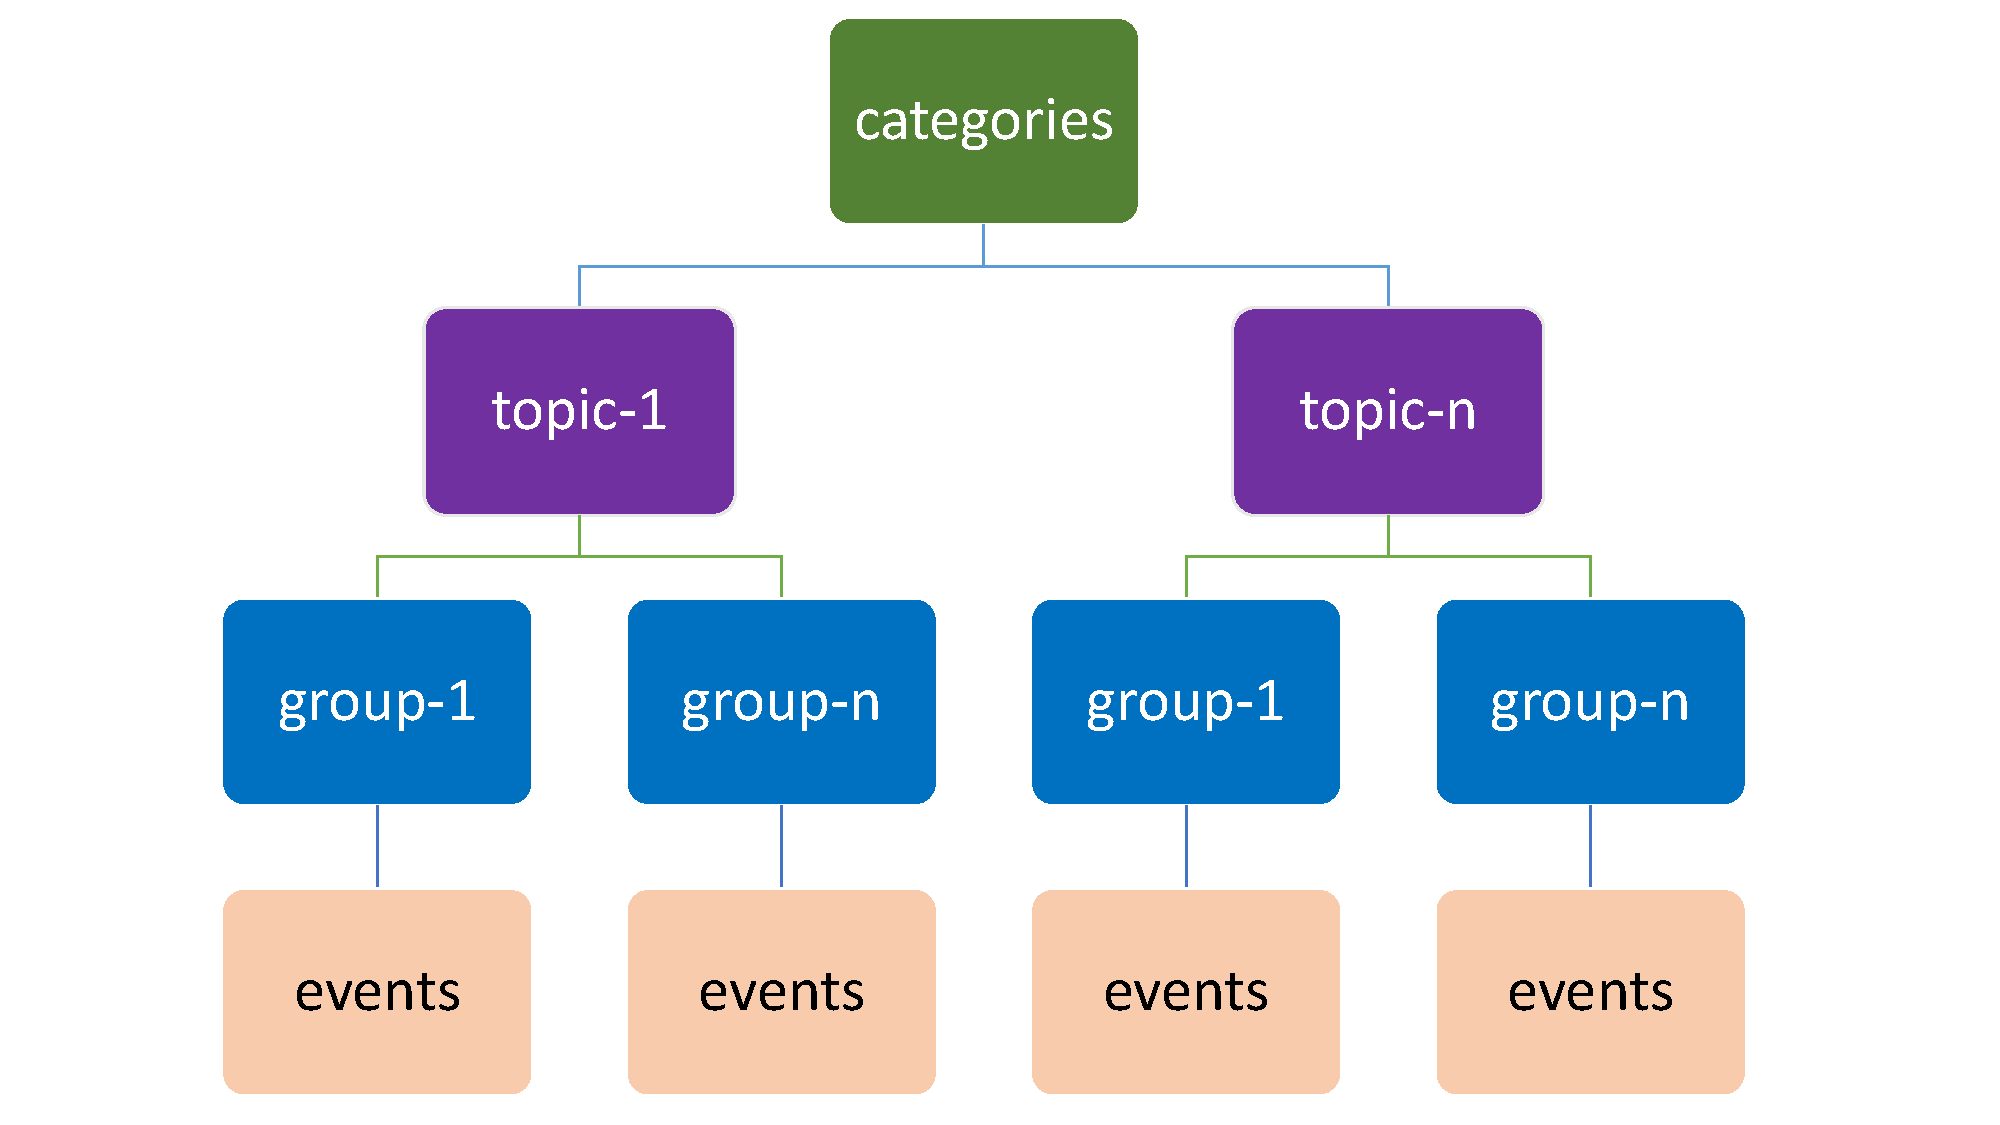
\includegraphics[width=1.0\columnwidth]{images/meetup_hierarchy.pdf}
  \caption{Meetup.com hierarchy}\label{F:hierarchy}
\end{figure}

\section{System Design}
This section describes the system design of this project.  We first describe the data pipeline (\$3.1) and the data model (\$3.2).  Finally, we describe the technology stack of this project (\$3.3). 

\subsection{Data Pipeline}
This section describes the high-level end-to-end data flow of the process.  The data is sourced from meetup.com that provides RESTful API for consumption.  We used Python libraries to consume this RESTful API  and loaded the data into HBase.  The data from HBase is consumed via Spark using third party library, analytics is performed within Spark and loads the aggregated data into HDFS.  We then use Python to read the data from HDFS and load it into MySQL.  Tableau is used as a visualization tool which will connect to MySQL and generate reports.  Figure~\ref{F:pipeline} shows the pictorial representation of the data pipeline.
\begin{figure}[!ht]
  \centering
      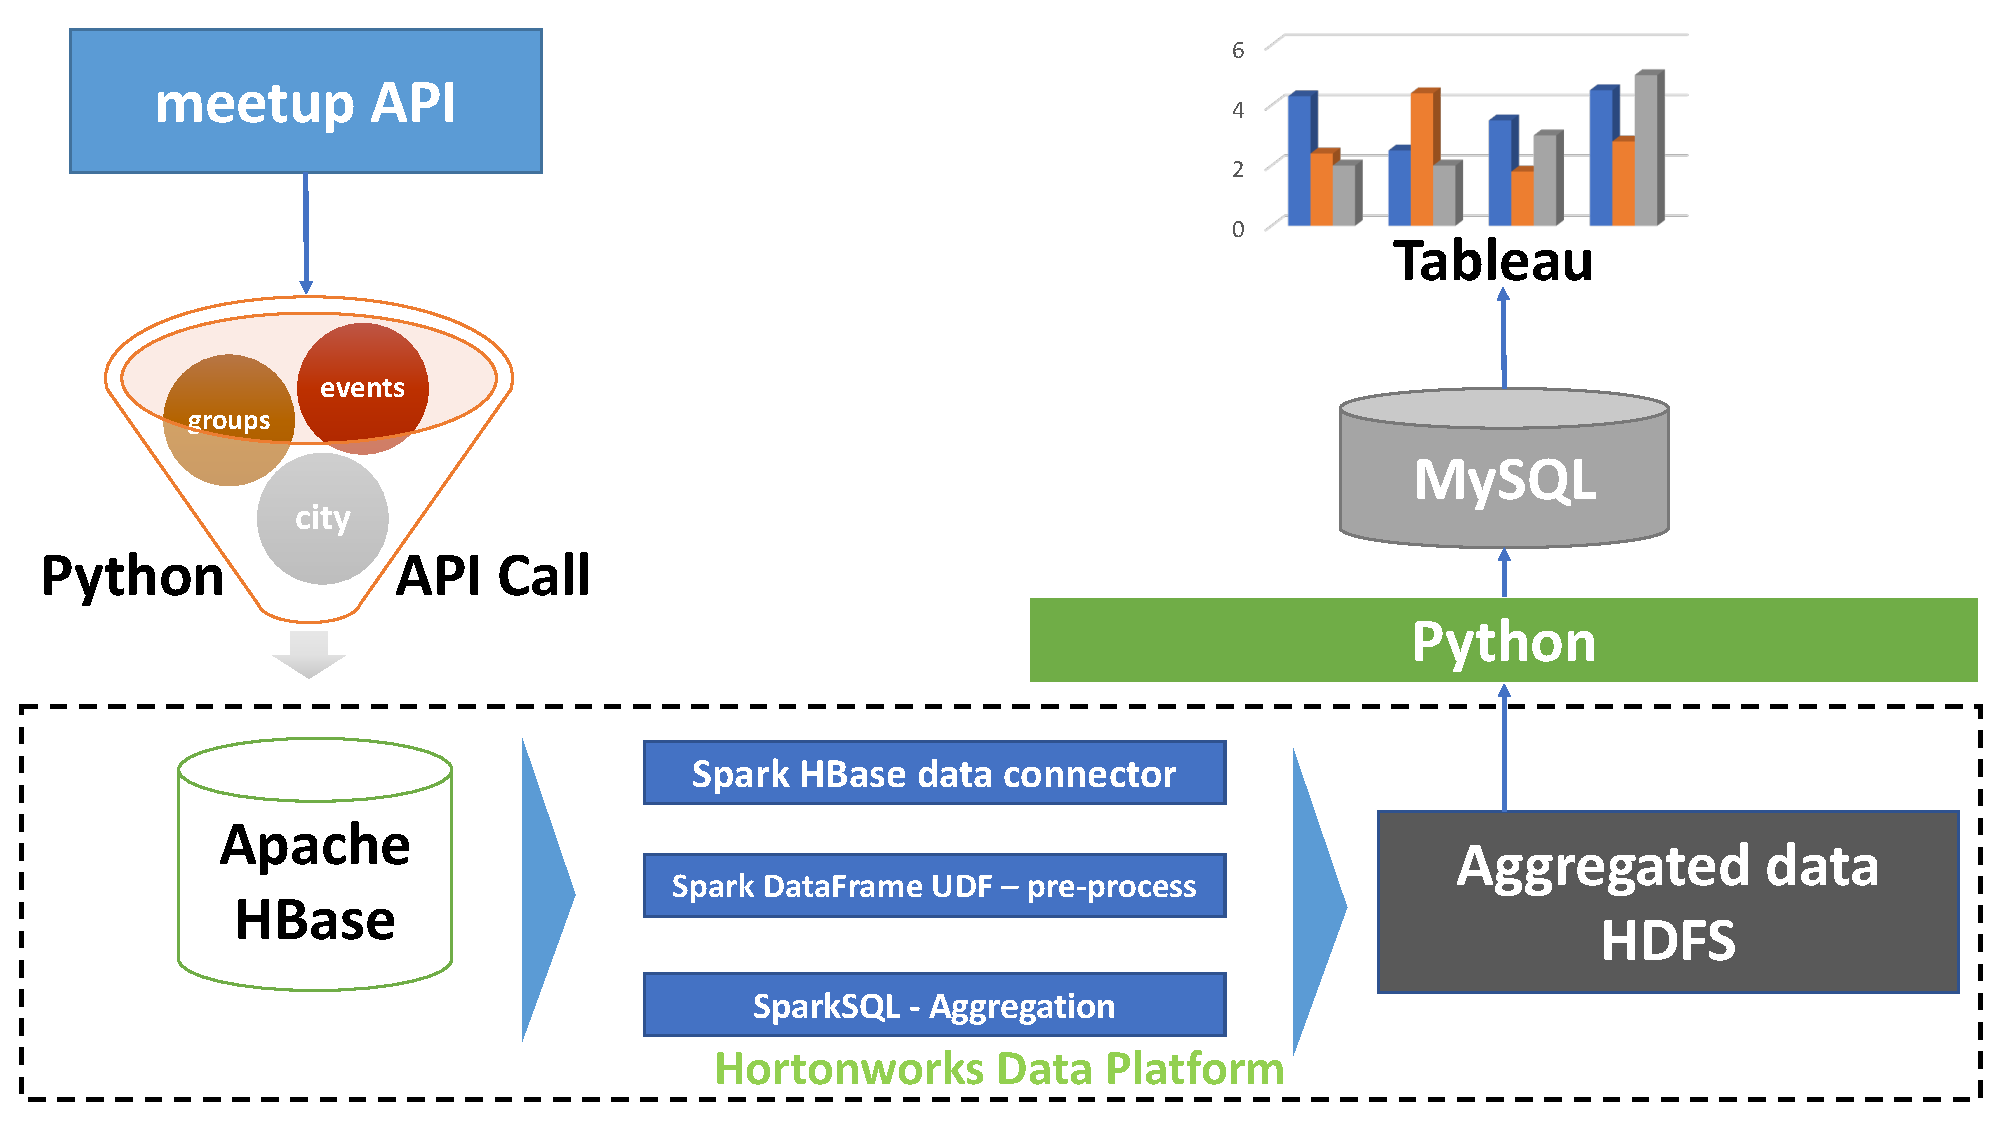
\includegraphics[width=1.0\columnwidth]{images/data_pipeline.pdf}
  \caption{Meetup Data Analysis - Data Pipeline}\label{F:pipeline}
\end{figure}

\subsection{Data Model}
This project has a Big Data NoSQL data store in HBase where the sourced data is loaded and MySQL is used to store the aggregated data.  Figure~\ref{F:datamodel} shows the different tables in HBase and aggregated/lookup tables in MySQL.  The source is providing numerous columns but we brainstormed and identified an optimal number of columns that would suffice our reporting needs.
\begin{figure}[!ht]
  \centering
      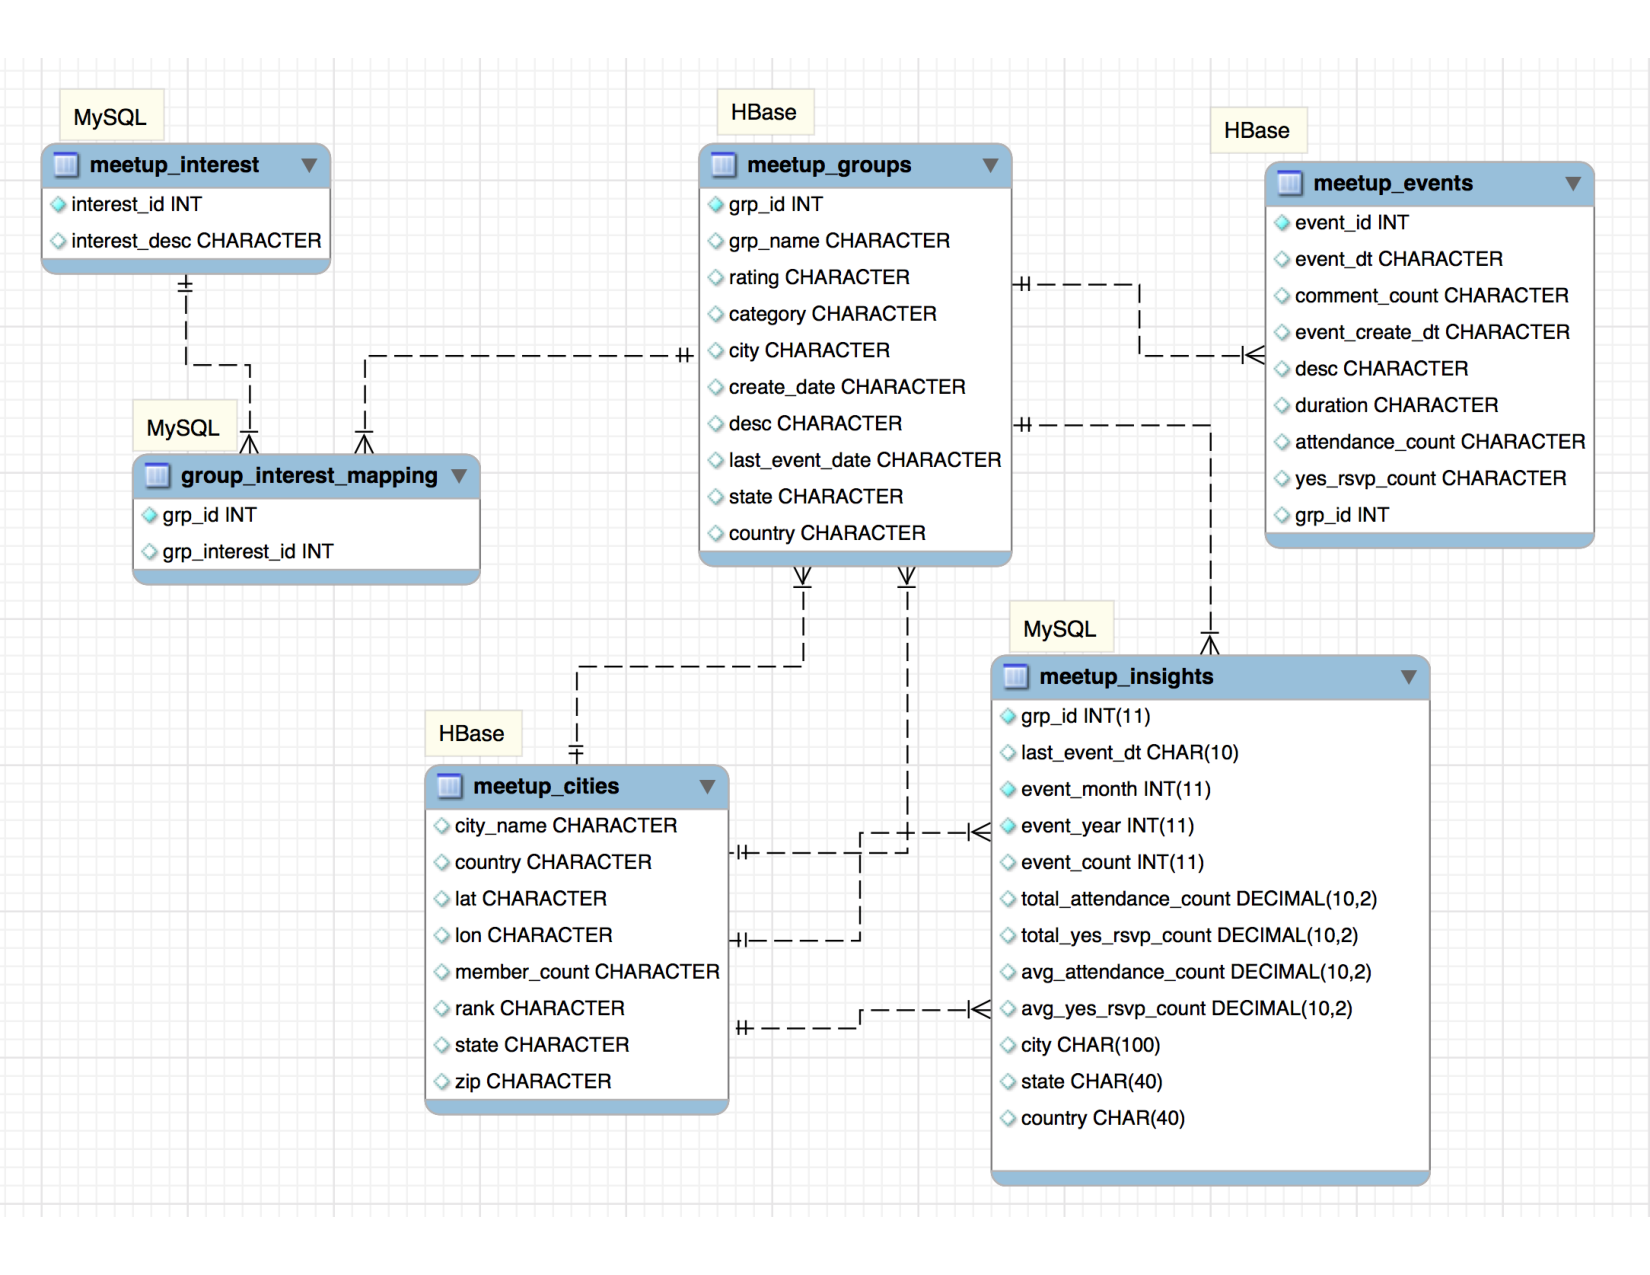
\includegraphics[width=1.0\columnwidth]{images/data_model.pdf}
  \caption{Meetup Data Analysis - Data Model}\label{F:datamodel}
\end{figure}

\subsection{Technology Stack}
This section describes different technologies that are involved in this project and the Hadoop cluster configuration details.  The development was done on a three-node cluster with Hortonworks Data Platform Community Edition \cite{www-hdp} as the Hadoop distribution.  Figure~\ref{F:dashboard} provides an overview of our platform. Figure~\ref{F:techstack} shows the pictorial representation of the technology stack of this project.  We have used trial version of Tableau Desktop \cite{www-tableau}.  The Table~\ref{T:softwareversion} shows the version of software used.

\begin{figure}[!ht]
  \centering
      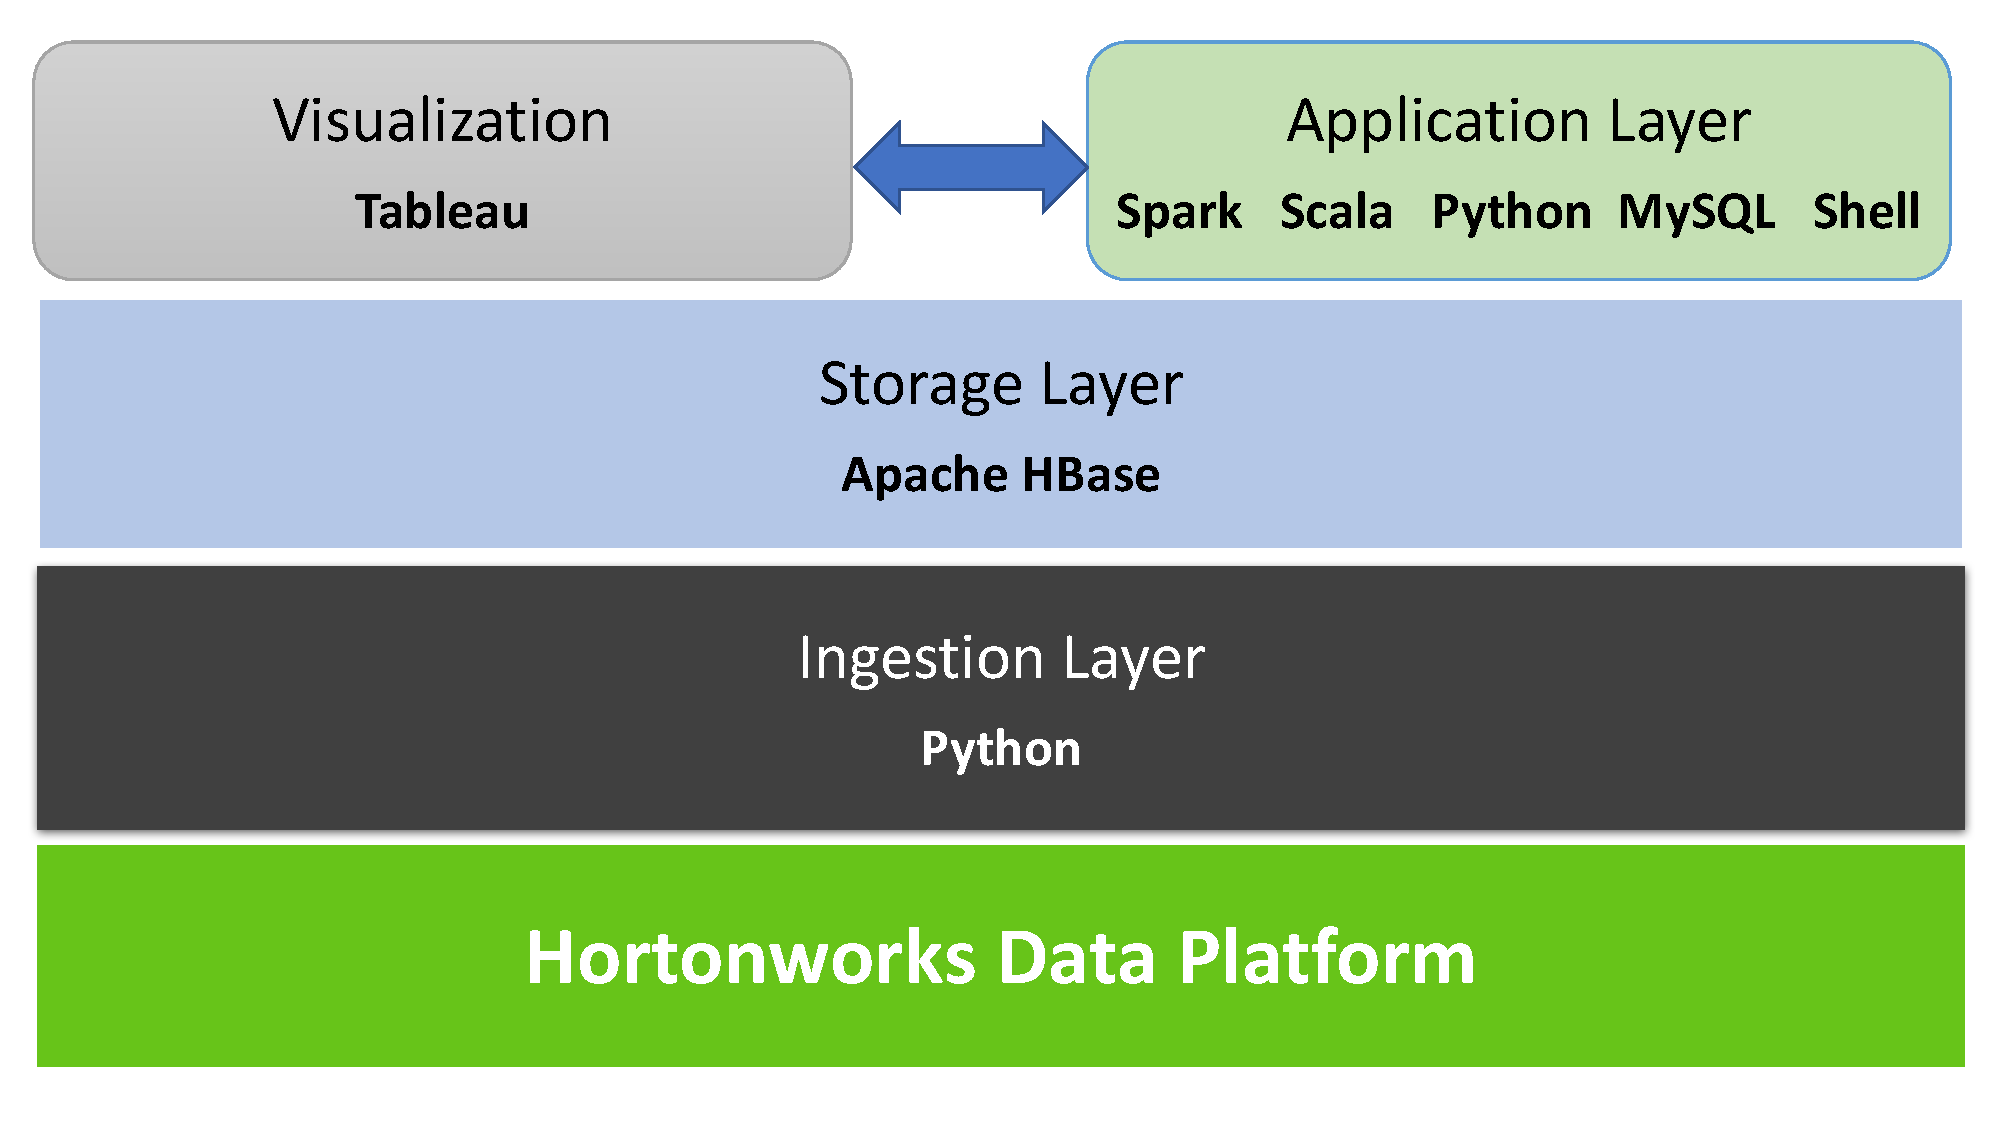
\includegraphics[width=1.0\columnwidth]{images/tech_stack.pdf}
  \caption{Technology Stack}\label{F:techstack}
\end{figure}

\begin{figure}[!ht]
  \centering
      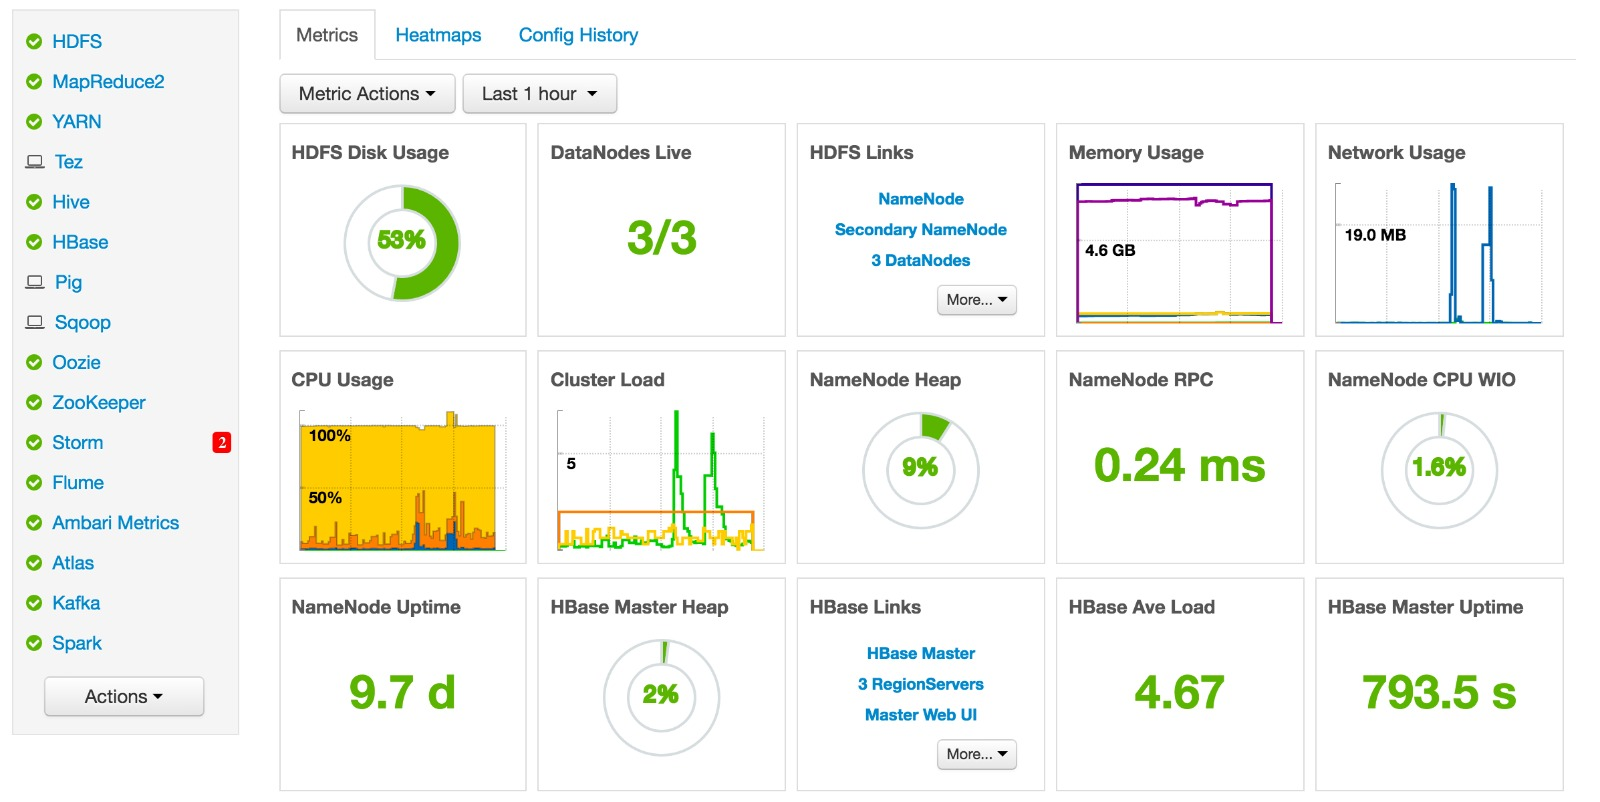
\includegraphics[width=1.0\columnwidth]{images/ambari_dashboard.jpeg}
  \caption{Hortonworks Data Platform}\label{F:dashboard}
\end{figure}

\begin{table}[htb]
\caption{Software versions}\label{T:softwareversion}
\bigskip
\begin{center}
\begin{tabular}{|c|c|c|} \hline S.No & Software Name & Version\\ \hline
1 & HDP platform & 2.4.2\\ \hline
2 & Apache Spark & 1.6.1\\ \hline
3 & Apache HBase & 1.1.2\\ \hline
4 & Python & 2.7\\ \hline
5 & Scala & 2.10\\ \hline
6 & MySQL & 5.7.16\\ \hline
7 & Tableau & 10.1.1\\ \hline
8 & Ubuntu OS & 14.0.4 LTS \\
\hline
\end{tabular}
\end{center}
\end{table}

We have used various third party libraries for this project.  Below is the list of libraries used.

\subsubsection{Spark-HBase connector}
We are using Hortonwork's Spark-HBase connector \cite{www-spark-hbase-connector} to connect to HBase from Spark.  This connector supports HBase dataframe API, which was very useful during our development, testing, and interactive query analysis in the REPL.  This is one of the main reasons to choose this connector over other HBase connectors and the other reason being its simplicity.  We just need to create a catalog that has table and column details and then we use the standard sqlContext with the required class from the connector's library.

\subsubsection{Spark-csv package}
Since we were using Spark 1.6.1 version for our development, we did not have a built-in function to write CSV files with a custom delimiter.  Hence, we used the spark-CSV \cite{www-spark-csv} built by Databricks, which provides this functionality along with the option to specify a flag whether we need a header or not in the output file.  This package is, however, built-in starting Spark 2.x.

\subsubsection{Joda-Time package}
The source data has datetime in epoch format and hence we had to change it to Gregorian date for which we leveraged the joda-time library \cite{www-spark-joda-time}.  We also used this library to fetch only the year and month part from the date as well.

\subsubsection{TypeSafe Config Package}
We wanted to parametrize the spark code without any values hard coded in it except for the column names.  The tables names, lookup file name, and the output path are all parameterized and to achieve this we had to use the typesafe config package \cite{www-typesafe-config} which gives the functionality to load the external configuration file with variables and values in it.  Once loaded, we can use the variable in the program.  This saved a lot of time during our development and testing by reducing the need to touch the code as the path and table names are configurable so we can create multiple test tables to test the program.

\subsubsection{SBT}
We used SBT \cite{www-sbt} to generate the fat jar.  We have included all these three third party libraries in the SBT dependency to generate the fat jar.  We used the third party libraries as a comma-separated list in the packages parameter on the REPL.

\subsubsection{HappyBase - Python HBase Connector}
To write data into HBase from Python, we used HappyBase module, which provides a Pythonic API to interact with HBase. Below the surface, HappyBase uses the Python Thrift library to connect to HBase using its Thrift gateway.

\section{Data Ingestion}
This section provides an overview of different meetup APIs, explains how data has been pulled, processed and stored. It also highlights the challenges faced during data ingestion.

\subsection{What is meetup API?}
The Meetup API \cite{www-meetup-api} provides RESTful HTTP and streaming interfaces for the developers and others with certain limitations.Typically, we can access it with a query to their server and they send back their data structured in different formats, usually in JSON format.
The API is a set of core methods and a common request format. These are combined to form a URL that returns the information we want.

Figure~\ref{F:requestresp} shows sample HTTP request and response for category API call.

\begin{figure}[!ht]
  \centering
      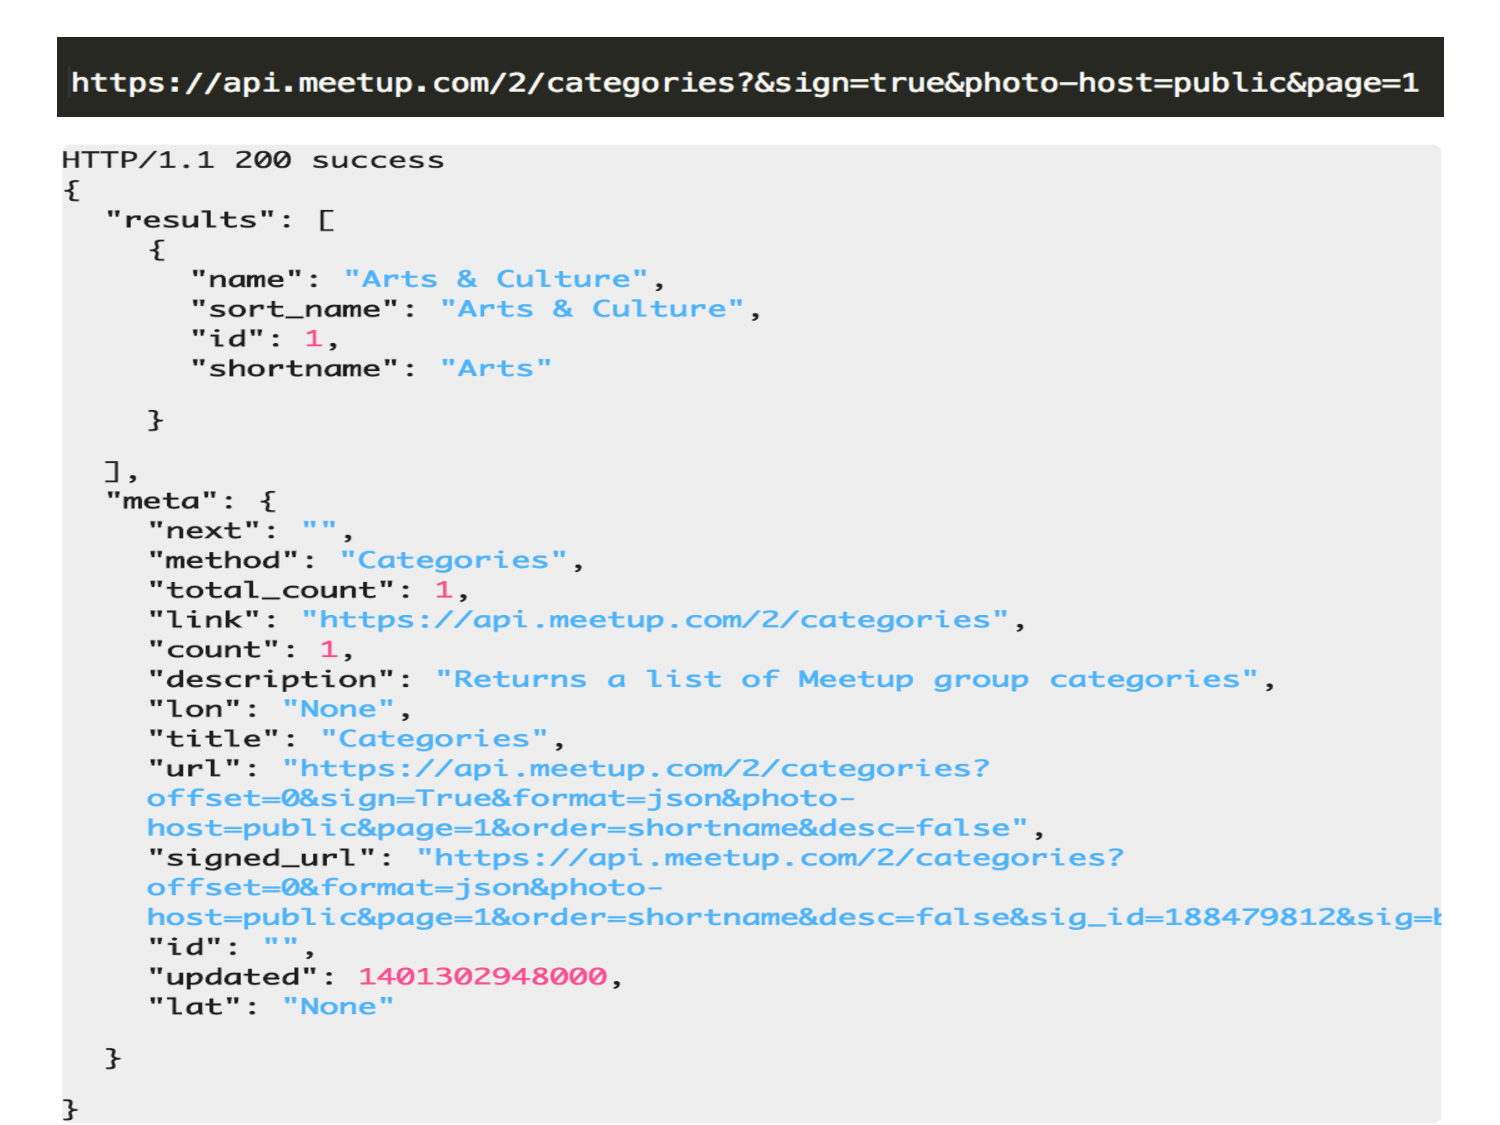
\includegraphics[width=1.0\columnwidth]{images/meetup_request_response.pdf}
  \caption{Meetup API Request and Response}\label{F:requestresp}
\end{figure}

\subsection{Meetup API Calls}
Meetup provides a number of APIs which can be used to pull different types of data. We used Category, Cities, Groups and Events APIs. We registered in meetup.com as a user and obtained an API key, which is used to authenticate the API calls.  We have used Python requests module to make API calls to fetch the data.  We first pulled information about cities in the US and India, then for each city, we have fetched details about the meetup groups, and finally, we fetched details about all the events hosted for each meetup groups.  Even though we pulled city details for all the cities in the US and India, we pulled groups and events details only for top cities in India and the US by population.

\subsection{Process API Response}
Responses have been parsed using Python JSON library. Once data is parsed, we do basic validation like null/empty check for the fields we are interested in.   We then persist the validated data into a NoSQL database which is HBase.

\subsection{Storing Data in HBase}
We stored the results in HBase.  Considering huge volume and  dynamic nature of meetup data, we choose a NoSQL database HBase to store our data.  HBase supports both low latency query and batch load, which has contributed to the decision of choosing HBase as the persistent data layer.

\begin{table}[htb]
\caption{Data Statistics}\label{T:statistics}
\bigskip
\begin{center}
\begin{tabular}{|c|c|} \hline Table Name & Record Count\\ \hline
meetup\_cities & 34,592 \\ \hline
meetup\_groups & 14,882 \\ \hline
meetup\_events & 289,239 \\
\hline\end{tabular}
\end{center}
\end{table}

\subsection{Data Pull Challenges}
Meetup APIs are subject to a limit on how many calls can be made per second (or minute, or another short time period), in order to protect servers from being overloaded and maintain a high quality of service to many clients. The limit that is tracked and enforced over a 60-second window. 

There are three important concepts here:
X-Rate-Limit-Limit \cite{www-data-pull-challenges} indicates how many calls our application may make per time window. This time window is currently 60 seconds for most of our APIs, but for the most reliable code, in this case, we have  uses the X-Rate-Limit-Reset header instead. X-Rate-Limit-Reset indicates when the current window ends, in seconds from the current time. X-Rate-Limit-Remaining indicates how many calls you have remaining in this window.

We have overcome this issue by monitoring X-Rate-Limit-Reset in the response header and introducing a short pause when this limit nears zero. The solution has ensured uninterrupted data flow overall.

\section{Data Analytics}
This section describes the analytics that was performed as part of this project.  It breaks the analytic process into multiple sections.  We first provide an overview of the analytics process and the list of topics that we did analysis on.  We then proceed with an explanation on how the group data and interest topics are tagged and then we talk about the aggregation that was carried out on the event data. 

\subsection{Overview}
We used Spark to carry out the analytics process.  We used the spark-HBase connector to load the data into Spark HBase dataframes.  We have predefined catalog for each of the tables in HBase such as groups, events, and city.  We also used a predefined list of interesting topics for our analysis.  We have used dataframes for standardizing and applying custom functions and we used SparkSQL for aggregations with Scala as the programming language.  We have used Spark Shell for our development and analysis.  We chose dataframe APIs as we were already familiar with the concept of dataframes and the another reason is that we can quickly build a table on top of the dataframes to do ad-hoc analysis using the standard SQL queries.

\subsection{List of interested topics}
We identified around 27 trending topics for our analysis. This list is completely configurable which means that there is no need of any code change if we want to add any new topic or remove existing topic.  Once the list is updated, all we need to do is, run the analytics process again and the results will be generated with the updated topic list.  Following are the list of topics that we have used for our analysis: python, scala, Julia, java, r, data science, machine learning, bitcoin, artificial intelligence, blockchain, HBase, hive, spark, Hadoop, big data, solr, pig, MongoDB, cloud, elasticsearch, neo4j, smart data, fast data, internet of things,, and DevOps.

\subsection{Interest - Group \& Event Mapping}
We have defined an integer key for each for topics that we have identified and placed it as a comma separated file in the cluster.  We loaded this file into map variable in the program and broadcasted it for optimal lookup.  We created a custom function which accepts the group name and group description as the parameter.  It removes all nonalphanumeric characters and squeezes the spaces and concatenates the name and description to a single column.  We then used the broadcasted map variable to look for the interesting topics in the concatenated column.  If found, we assign the key in a comma separated variable for all the identified topics for that column.  We then pivot this comma separated value into rows for each group and write it into a comma separated file using the databricks spark-CSV library.  In a similar way, we identify the interest mapping for the event data and write it into a comma separated file.

\subsection{Data Aggregation}
We did date formatting for the event date column as the date from source is in epoch format.  We have created an user-defined function to convert the date to Gregorian date format using the joda-time package.  We also derived month and year columns from the processed date.  We used the HBase dataframe to pull the event and city data.  We then aggregated the data using SparkSQL based on group id, month and year to identify the number of events that happened for a given group, attendance count, RSVP count, and the date when the last event took place for each group as it will help to identify whether the group is still active or not. The aggregated data will be loaded into HDFS in a CSV file.  Figure~\ref{F:sampledata} shows the sample aggregated data.  The aggregated data from HDFS is then loaded into MySQL using Python.

\begin{figure}[!ht]
  \centering
      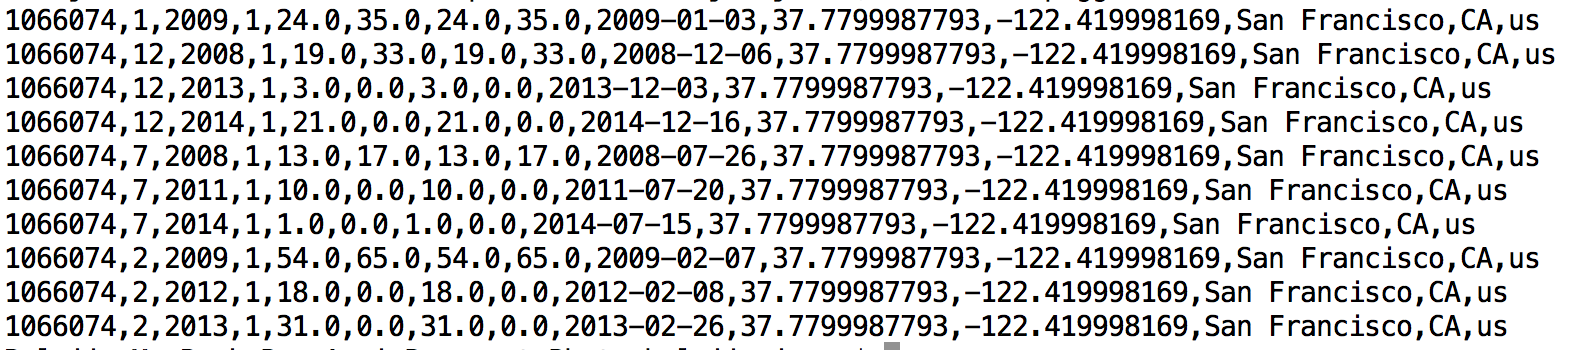
\includegraphics[width=1.0\columnwidth]{images/sample_aggregated_data.png}
  \caption{Sample Aggregated Data}\label{F:sampledata}
\end{figure}

\subsection{Data Analytics Implementation}
The entire aggregation is implemented in Spark and Scala.  Automation is done using shell scripts.  The fat jar is created for easier deployment and automation and parameters are configuration file driven to make it easy to move across different clusters.  The configuration file has output file path, master URL, deployment mode, and HBase configuration folder path.  The parameterized scripts were helpful during our testing to move between local mode and cluster mode without code change.

\begin{figure}[!ht]
  \centering
      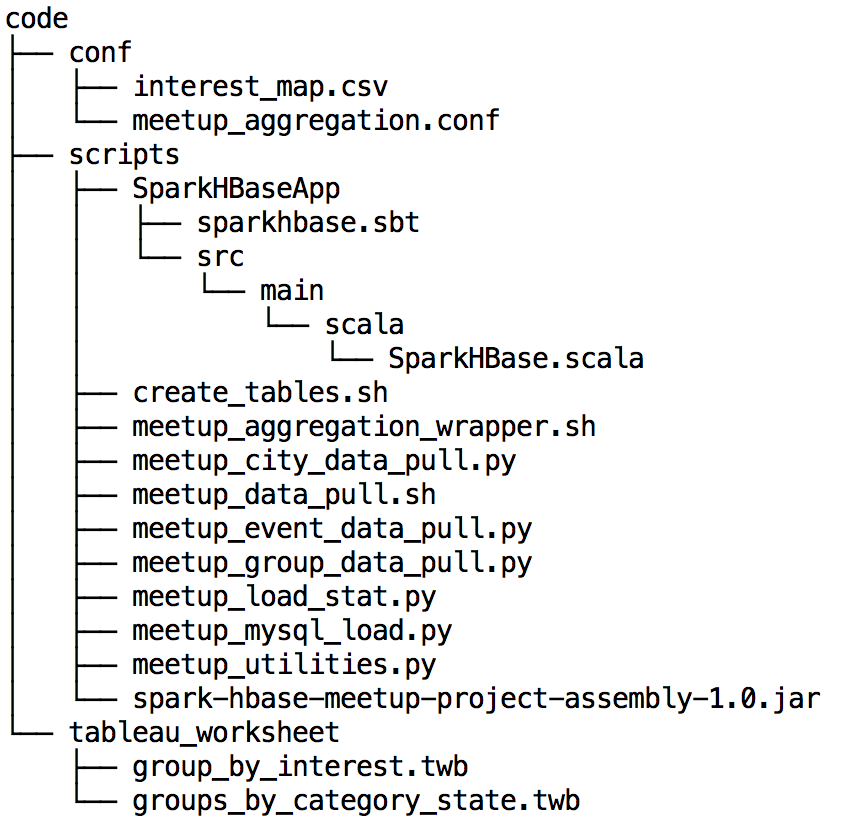
\includegraphics[width=1.0\columnwidth]{images/code_directory_tree.png}
  \caption{Project Folder Structure}\label{F:codetree}
\end{figure}

\section{Visualization}
We used Tableau to build our visualization given the ease of installation and usability.  This section describes the types of visualization and experimental results in details.  We used MySQL \& CSV as the source for Tableau.

\subsection{Temporal Analysis}
We would like to first start with our analysis on the growth of the meetup platform on India and the United States that may show the motivation behind this project.  We used the derived data that has the year and event counts based on groups to perform this analysis and to plot the growth chart.  The growth chart was plotted with the year on the x-axis and event counts on the y-axis.  The analysis showed that the meetup platform has exponential growth over the last couple of years.  The growth of this platform in India is still showing positive signs whereas the growth in the United States is slowing down.  Figure~\ref{F: meetupgrowth} shows the growth chart dashboard in Tableau that shows the overall meetup growth and the growth in India and the United States separately.
\begin{figure*}[p]
  \centering
      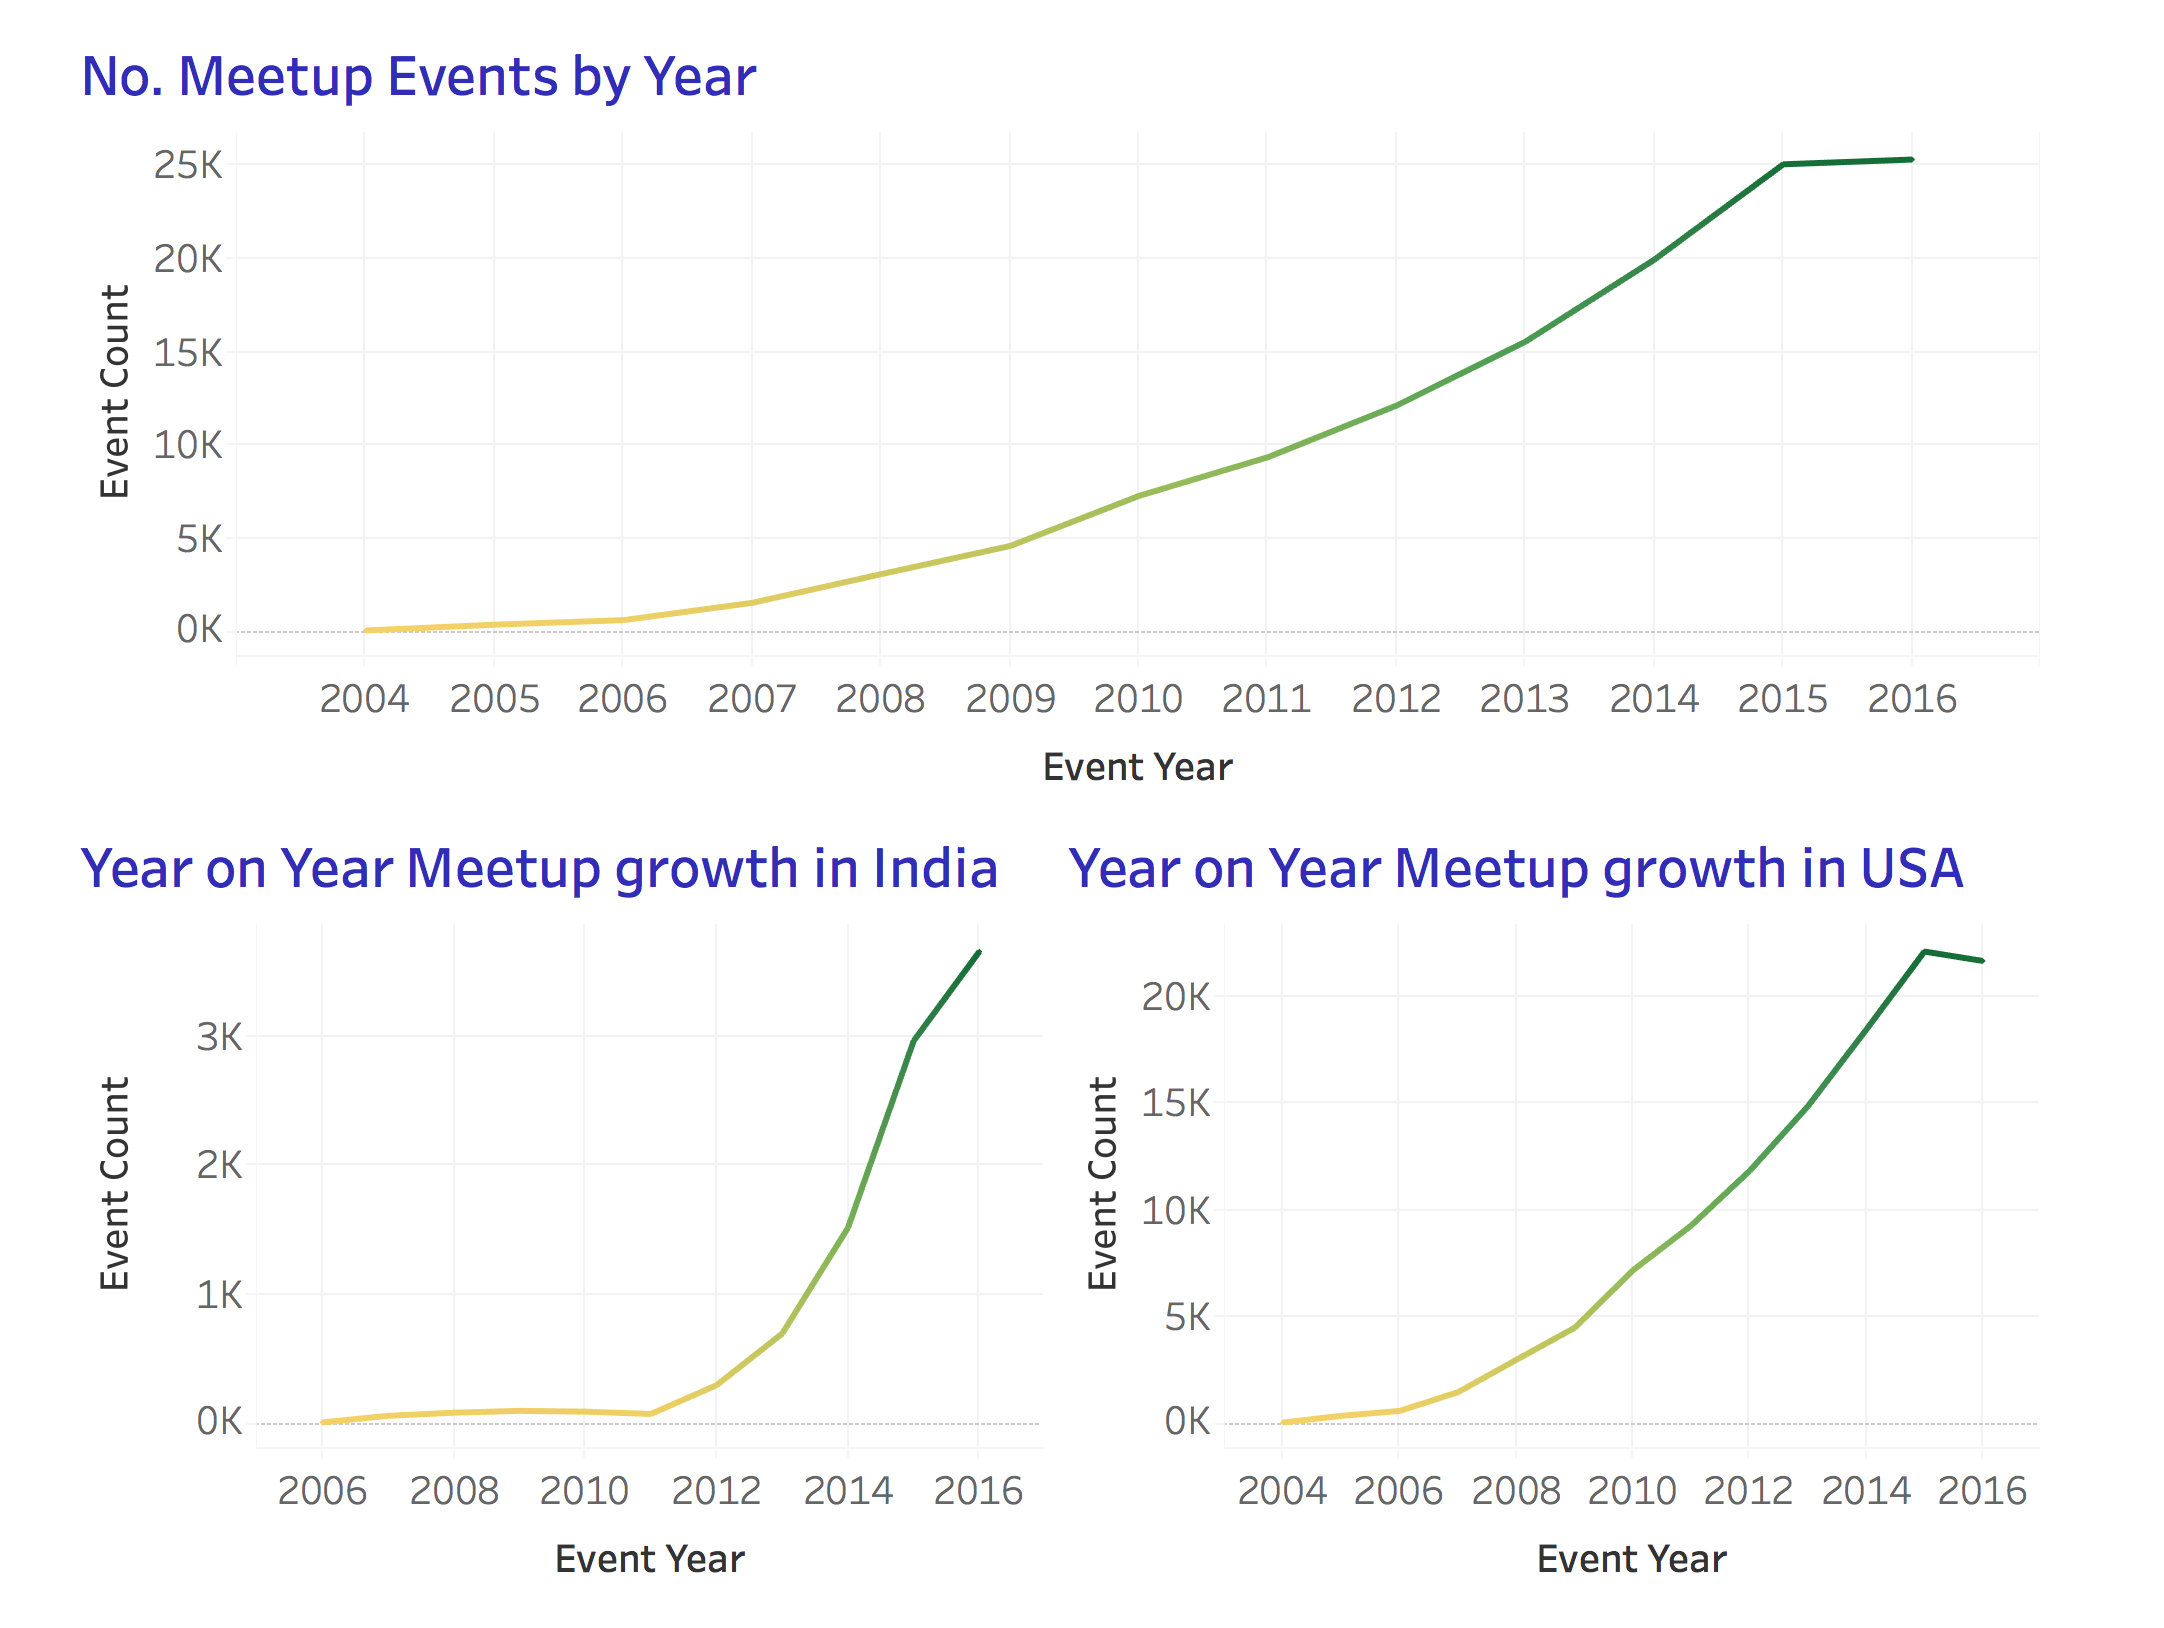
\includegraphics[width=0.9\linewidth,height=10cm]{images/tableau_images/year_on_year_growth-dashboard.png}
  \caption{Meetup popularity Year on Year Growth}\label{F: meetupgrowth}
\end{figure*}

\begin{figure*}[p]
  \centering
      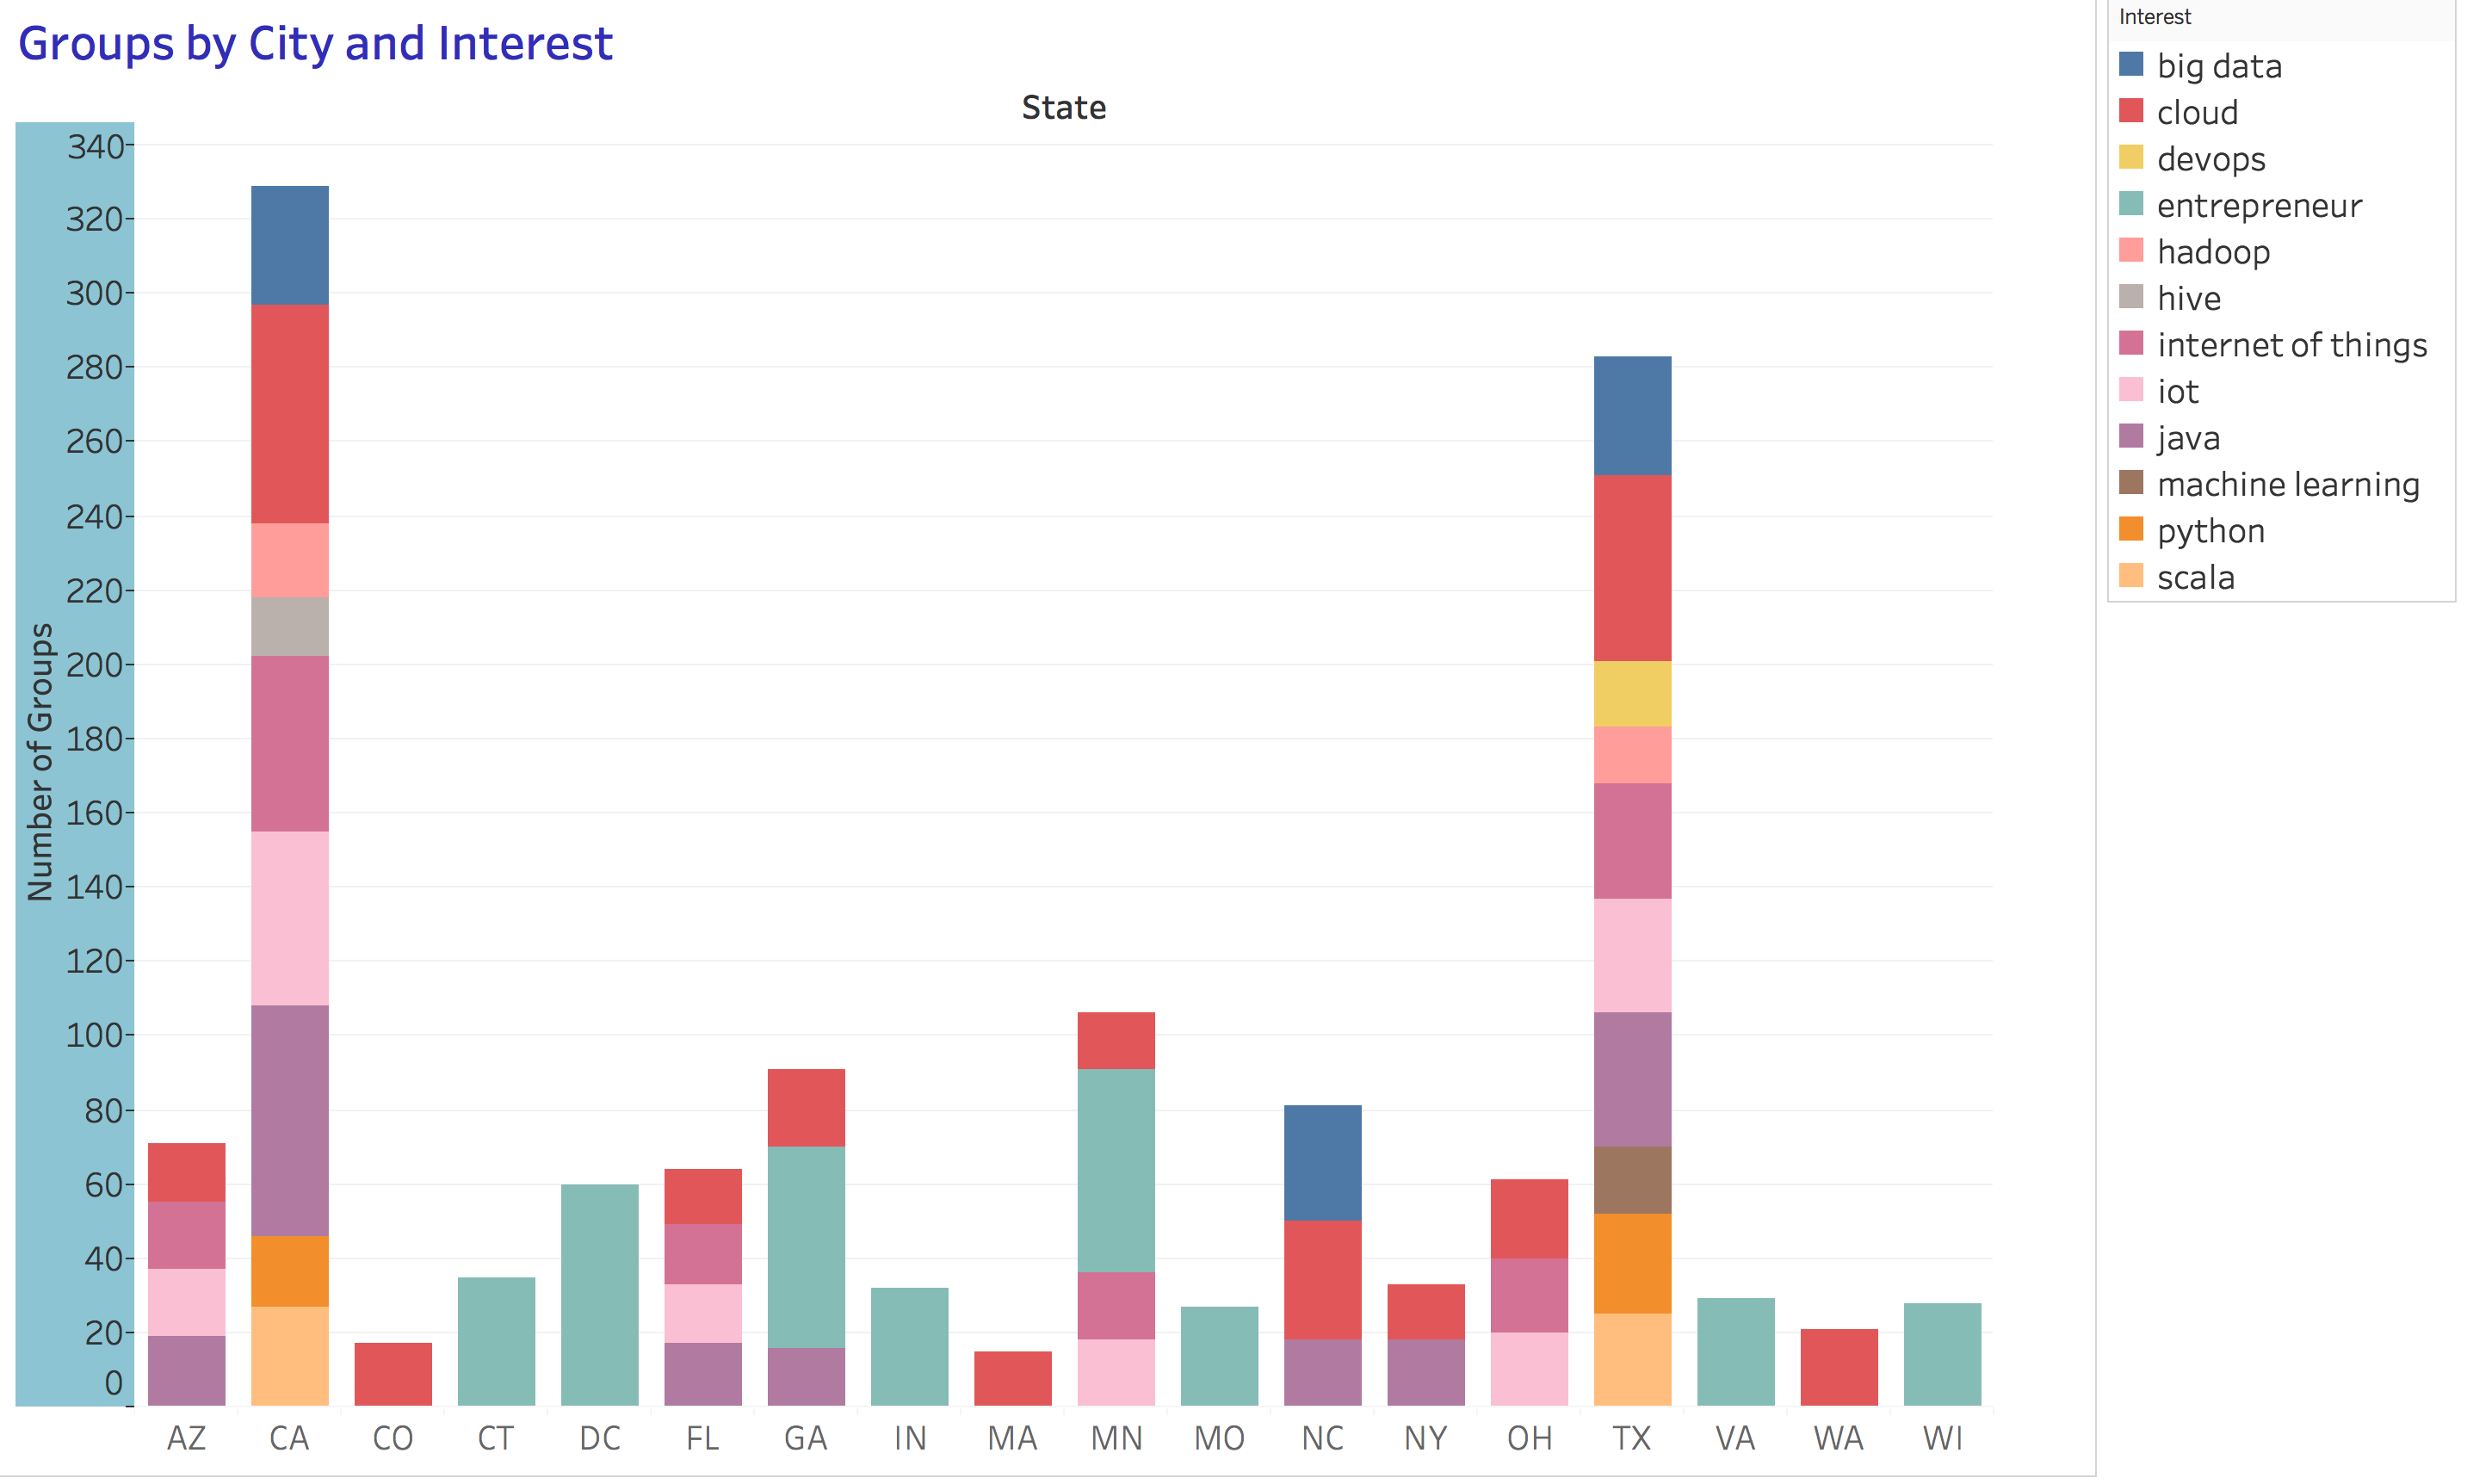
\includegraphics[width=0.9\linewidth,height=10cm]{images/tableau_images/groups_by_city_and_interest.png}
  \caption{Groups by City and Interest}\label{F:groupbycitynint}
\end{figure*}

\subsection{Geospatial Analysis}
This section describes the geospatial analysis performed and the experimental results.  The first section describes the popularity of meetup by state and the next section shows the most active cities in the meetup across the United States and India.  Analysis by the state was possible only for the United States as the meetup platform provides state value only for the United States and Canada whereas it provides a null value for other countries in the world.

\subsubsection{Popularity by State and Category}
We used the category, state, and the group data to perform the analysis.  We aggregated the number of groups by state and categories of our interest (Carrier \& Business and Tech).  Figure~\ref{F:groupbycat} shows the geographical heat map by category and state.  It was interesting to note that California has more meetup groups for both the categories than any other state in the United States.  Since the analysis was performed with a subset of data, we were not able to cover all the states and hence the comparison we provided is within the states for which we had data.
\begin{figure*}[p]
  \centering
      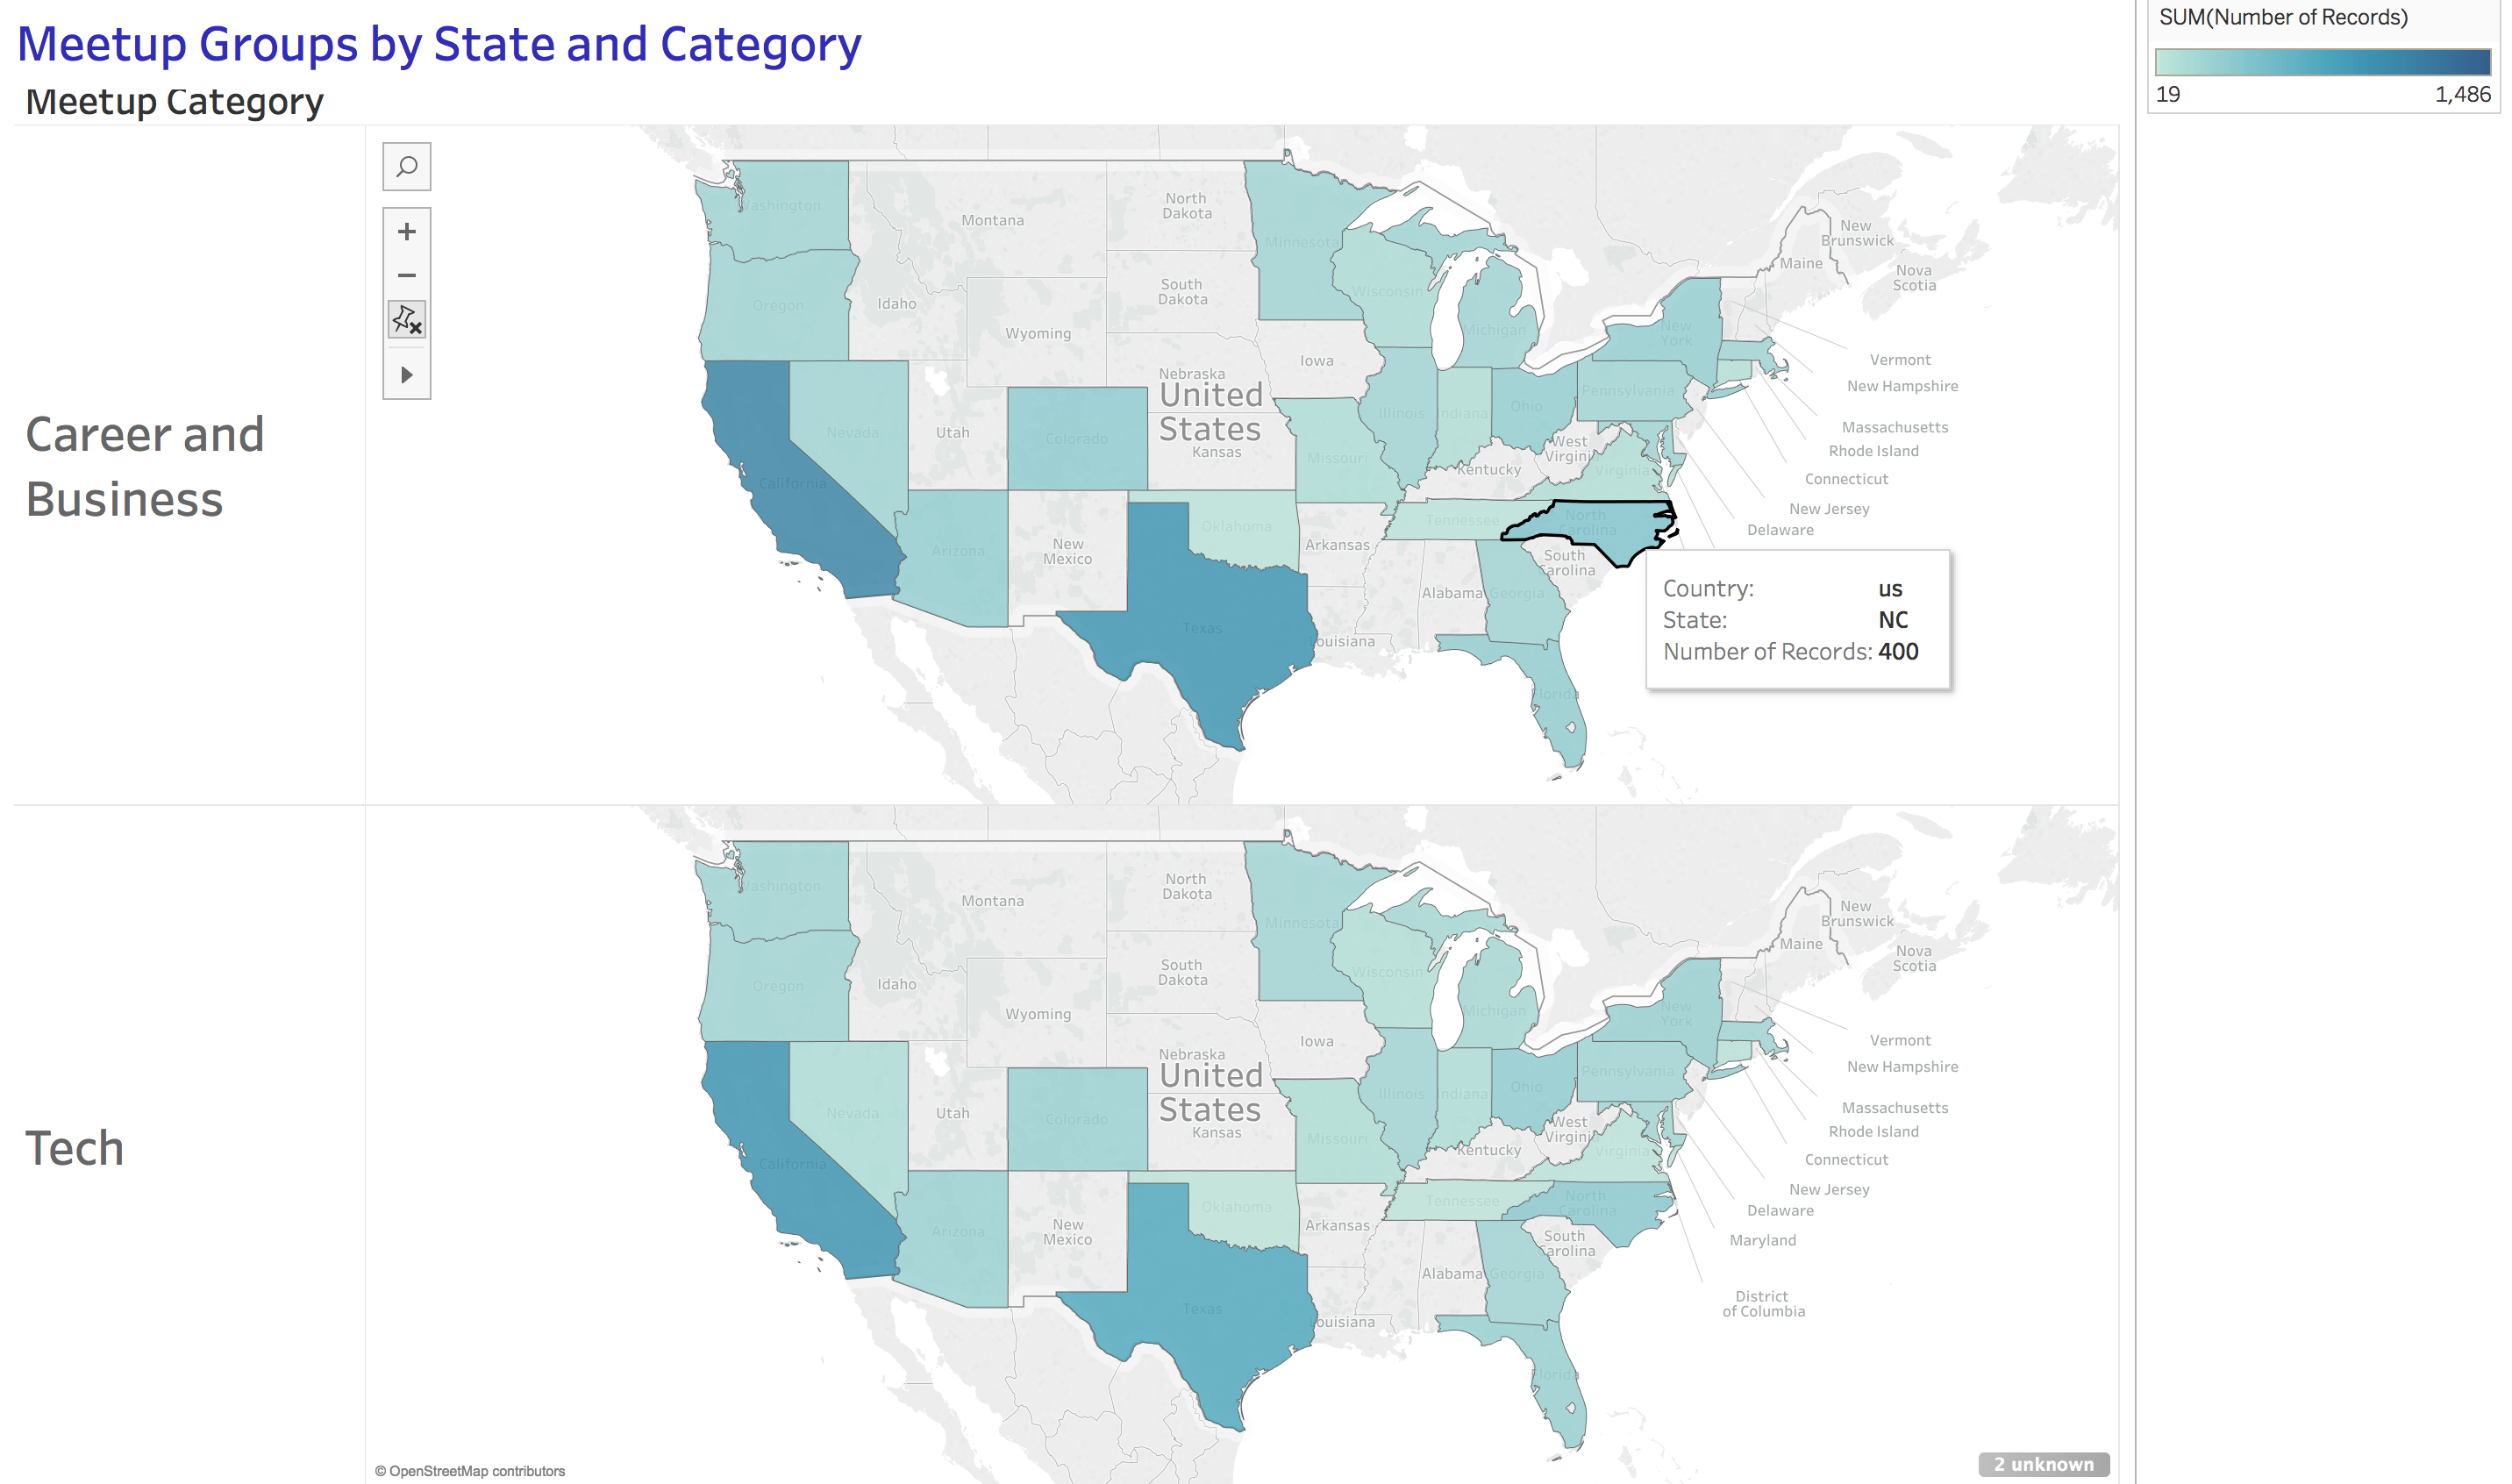
\includegraphics[width=0.9\linewidth]{images/tableau_images/groups_by_category_state.png}
  \caption{Groups by Category State}\label{F:groupbycat}
\end{figure*}

\begin{figure*}[p]
  \centering
      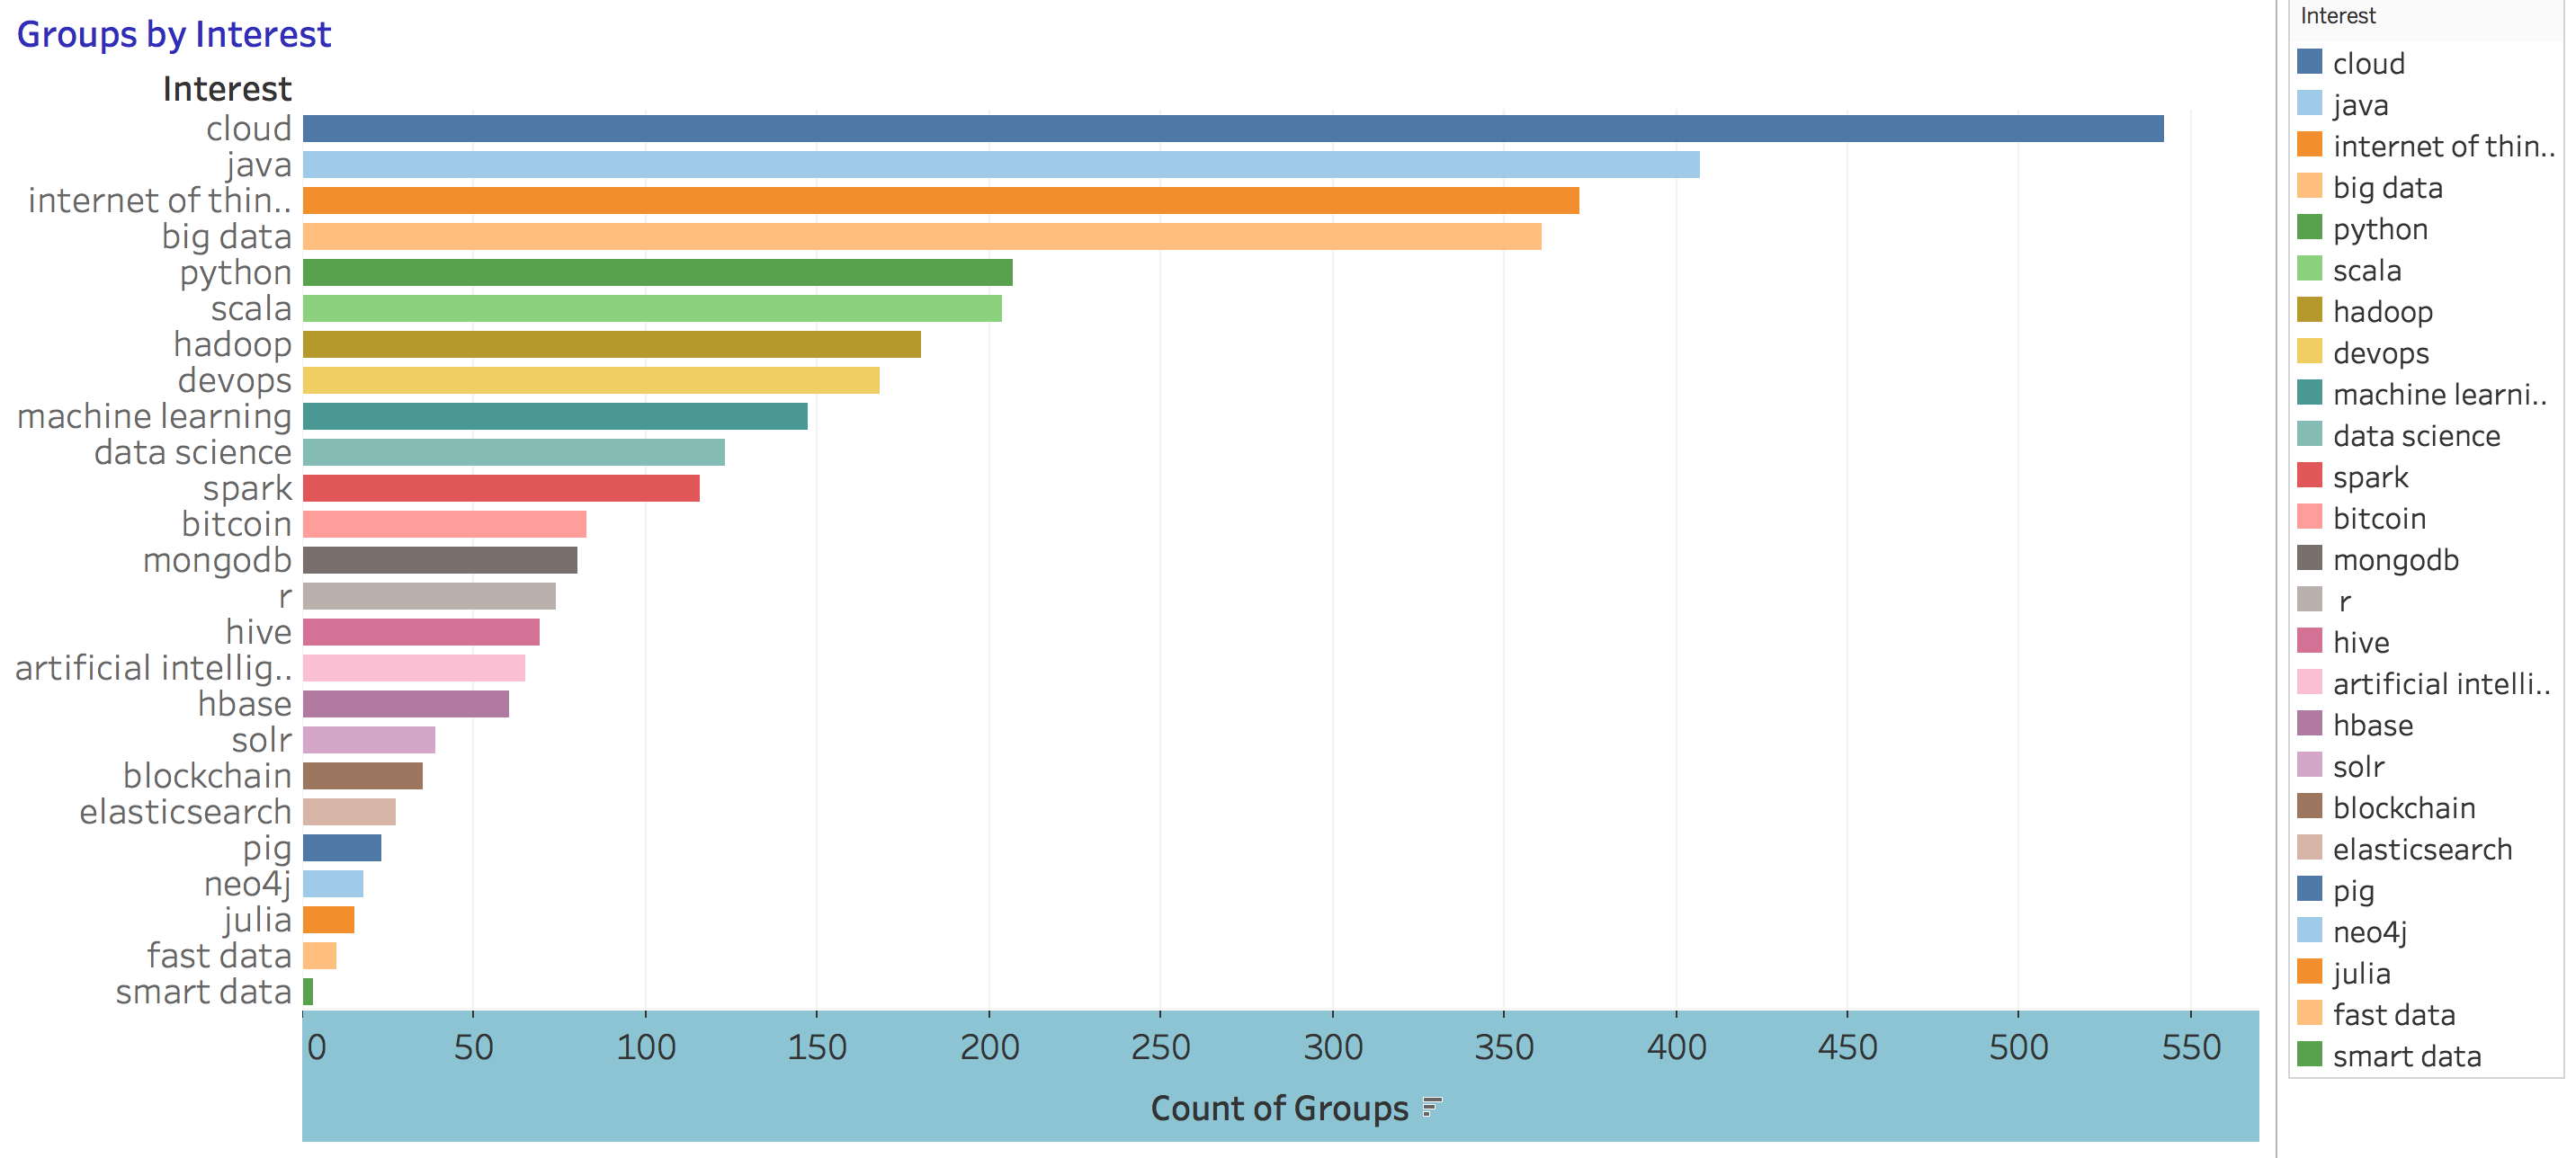
\includegraphics[width=0.9\linewidth]{images/tableau_images/groups_by_interest.png}
  \caption{Groups by Interest}\label{F:groupsbyint}
\end{figure*}

We have also provided state-wise analysis and popularity of tech groups stacked by interest.  Figure~\ref{F:groupbycitynint} shows the stacked bar chart of this analysis.

\subsubsection{Active Cities Analysis}
We used the aggregated the data again to find out which cities are more active in terms of conducting events in the United States.  Having more meetup groups in a city does not always mean that they are active and hence we identified the number of events conducted under each group and aggregated it by cities that shows the active cities in the meetup.  Figure~\ref{F:activecities} shows the bubble chart of more active cities in the meetup.
\begin{figure*}[p]
  \centering
      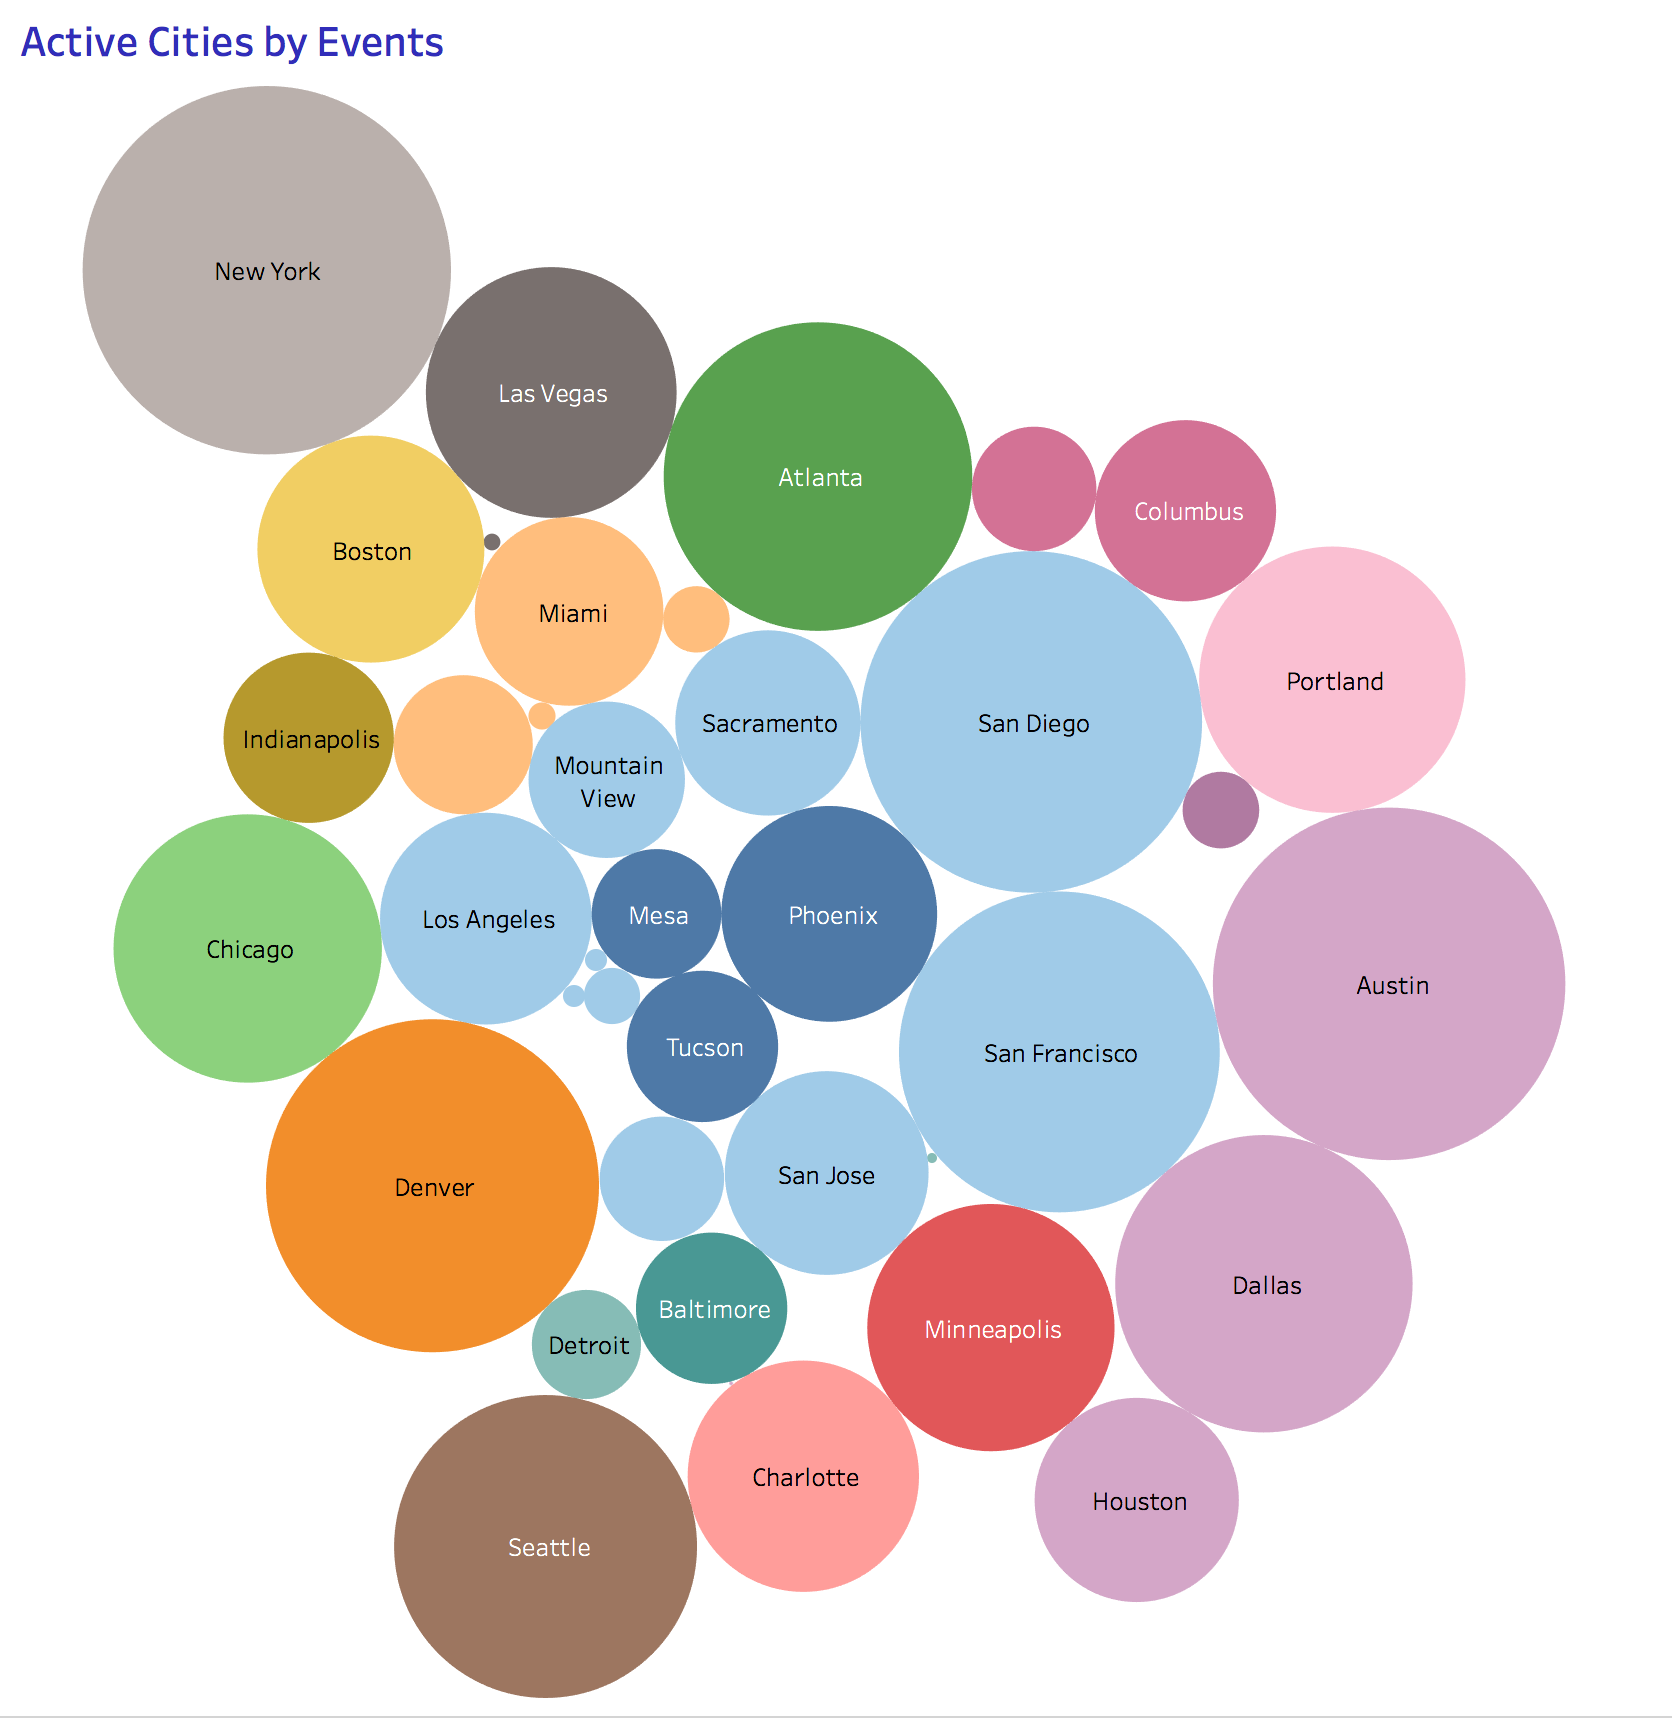
\includegraphics[width=1.0\textwidth]{images/tableau_images/active_cities_by_event_v2.png}
  \caption{Active Cities by Events}\label{F:activecities}
\end{figure*}

\section{Analysis by Interest}
The analysis was performed on the group and interest mapping data.  Figure~\ref{F:groupsbyint} shows which topics have more meetup groups in the descending order.  It was interesting to note that Cloud, Java, and Internet of Things are the top three topics that have more meetup groups.   This shows the growth of cloud computing and Internet of Things.

\section{Development}
We are a team of two members located in different locations and hence we used gitlab to push code updates.  The project is modularized and Table~\ref{T:tasks} shows the task breakdown by us.  We used Google Hangout for all the meetings including screen-sharing sessions.
\begin{table}[htb]
\caption{Tasks Breakdown}\label{T:tasks}
\bigskip
\begin{center}
\begin{tabular}{|p{3cm}|p{2cm}|p{3cm}|} \hline 
Tasks & Participants & Communication Mode\\ \hline
Analysis \& Design & Malabika, Balaji & Google Hangout\\ \hline
Data Model & Malabika, Balaji & Google Hangout\\ \hline
Ingestion Module & Malabika & gitlab\\ \hline
Analytics Module & Balaji & gitlab\\ \hline
Visualization Module & Malabika, Balaji & Google Hangout\\ \hline
report & Malabika, Balaji & Shared Sharelatex\\ 
\hline\end{tabular}
\end{center}
\end{table}

\section{Setup}
The project is organized as per the course requirements with code directory at the top level.  Figure~\ref{F:codetree} shows how the code directory is organized.  The scala source code is inside the SparkHBaseApp folder.

\section{Future Improvements}
We have used a simple user-defined function to identify interest topics among groups and events.  We could use machine learning libraries in Spark to do a more sophisticated text analysis or by using other third party libraries through which we can get more insights.  We can also use Spark streaming to pull the RSVP stream data for specific events to show the trending event topics.  We could also perform analysis to find out the commonly used words in technical groups.


\bibliographystyle{IEEEtran}
\bibliography{references}

%\balancecolumns 

\end{document}